% Options for packages loaded elsewhere
\PassOptionsToPackage{unicode}{hyperref}
\PassOptionsToPackage{hyphens}{url}
%
\documentclass[
]{article}
\usepackage{amsmath,amssymb}
\usepackage{iftex}
\ifPDFTeX
  \usepackage[T1]{fontenc}
  \usepackage[utf8]{inputenc}
  \usepackage{textcomp} % provide euro and other symbols
\else % if luatex or xetex
  \usepackage{unicode-math} % this also loads fontspec
  \defaultfontfeatures{Scale=MatchLowercase}
  \defaultfontfeatures[\rmfamily]{Ligatures=TeX,Scale=1}
\fi
\usepackage{lmodern}
\ifPDFTeX\else
  % xetex/luatex font selection
\fi
% Use upquote if available, for straight quotes in verbatim environments
\IfFileExists{upquote.sty}{\usepackage{upquote}}{}
\IfFileExists{microtype.sty}{% use microtype if available
  \usepackage[]{microtype}
  \UseMicrotypeSet[protrusion]{basicmath} % disable protrusion for tt fonts
}{}
\makeatletter
\@ifundefined{KOMAClassName}{% if non-KOMA class
  \IfFileExists{parskip.sty}{%
    \usepackage{parskip}
  }{% else
    \setlength{\parindent}{0pt}
    \setlength{\parskip}{6pt plus 2pt minus 1pt}}
}{% if KOMA class
  \KOMAoptions{parskip=half}}
\makeatother
\usepackage{xcolor}
\usepackage[margin=1in]{geometry}
\usepackage{color}
\usepackage{fancyvrb}
\newcommand{\VerbBar}{|}
\newcommand{\VERB}{\Verb[commandchars=\\\{\}]}
\DefineVerbatimEnvironment{Highlighting}{Verbatim}{commandchars=\\\{\}}
% Add ',fontsize=\small' for more characters per line
\usepackage{framed}
\definecolor{shadecolor}{RGB}{248,248,248}
\newenvironment{Shaded}{\begin{snugshade}}{\end{snugshade}}
\newcommand{\AlertTok}[1]{\textcolor[rgb]{0.94,0.16,0.16}{#1}}
\newcommand{\AnnotationTok}[1]{\textcolor[rgb]{0.56,0.35,0.01}{\textbf{\textit{#1}}}}
\newcommand{\AttributeTok}[1]{\textcolor[rgb]{0.13,0.29,0.53}{#1}}
\newcommand{\BaseNTok}[1]{\textcolor[rgb]{0.00,0.00,0.81}{#1}}
\newcommand{\BuiltInTok}[1]{#1}
\newcommand{\CharTok}[1]{\textcolor[rgb]{0.31,0.60,0.02}{#1}}
\newcommand{\CommentTok}[1]{\textcolor[rgb]{0.56,0.35,0.01}{\textit{#1}}}
\newcommand{\CommentVarTok}[1]{\textcolor[rgb]{0.56,0.35,0.01}{\textbf{\textit{#1}}}}
\newcommand{\ConstantTok}[1]{\textcolor[rgb]{0.56,0.35,0.01}{#1}}
\newcommand{\ControlFlowTok}[1]{\textcolor[rgb]{0.13,0.29,0.53}{\textbf{#1}}}
\newcommand{\DataTypeTok}[1]{\textcolor[rgb]{0.13,0.29,0.53}{#1}}
\newcommand{\DecValTok}[1]{\textcolor[rgb]{0.00,0.00,0.81}{#1}}
\newcommand{\DocumentationTok}[1]{\textcolor[rgb]{0.56,0.35,0.01}{\textbf{\textit{#1}}}}
\newcommand{\ErrorTok}[1]{\textcolor[rgb]{0.64,0.00,0.00}{\textbf{#1}}}
\newcommand{\ExtensionTok}[1]{#1}
\newcommand{\FloatTok}[1]{\textcolor[rgb]{0.00,0.00,0.81}{#1}}
\newcommand{\FunctionTok}[1]{\textcolor[rgb]{0.13,0.29,0.53}{\textbf{#1}}}
\newcommand{\ImportTok}[1]{#1}
\newcommand{\InformationTok}[1]{\textcolor[rgb]{0.56,0.35,0.01}{\textbf{\textit{#1}}}}
\newcommand{\KeywordTok}[1]{\textcolor[rgb]{0.13,0.29,0.53}{\textbf{#1}}}
\newcommand{\NormalTok}[1]{#1}
\newcommand{\OperatorTok}[1]{\textcolor[rgb]{0.81,0.36,0.00}{\textbf{#1}}}
\newcommand{\OtherTok}[1]{\textcolor[rgb]{0.56,0.35,0.01}{#1}}
\newcommand{\PreprocessorTok}[1]{\textcolor[rgb]{0.56,0.35,0.01}{\textit{#1}}}
\newcommand{\RegionMarkerTok}[1]{#1}
\newcommand{\SpecialCharTok}[1]{\textcolor[rgb]{0.81,0.36,0.00}{\textbf{#1}}}
\newcommand{\SpecialStringTok}[1]{\textcolor[rgb]{0.31,0.60,0.02}{#1}}
\newcommand{\StringTok}[1]{\textcolor[rgb]{0.31,0.60,0.02}{#1}}
\newcommand{\VariableTok}[1]{\textcolor[rgb]{0.00,0.00,0.00}{#1}}
\newcommand{\VerbatimStringTok}[1]{\textcolor[rgb]{0.31,0.60,0.02}{#1}}
\newcommand{\WarningTok}[1]{\textcolor[rgb]{0.56,0.35,0.01}{\textbf{\textit{#1}}}}
\usepackage{graphicx}
\makeatletter
\def\maxwidth{\ifdim\Gin@nat@width>\linewidth\linewidth\else\Gin@nat@width\fi}
\def\maxheight{\ifdim\Gin@nat@height>\textheight\textheight\else\Gin@nat@height\fi}
\makeatother
% Scale images if necessary, so that they will not overflow the page
% margins by default, and it is still possible to overwrite the defaults
% using explicit options in \includegraphics[width, height, ...]{}
\setkeys{Gin}{width=\maxwidth,height=\maxheight,keepaspectratio}
% Set default figure placement to htbp
\makeatletter
\def\fps@figure{htbp}
\makeatother
\setlength{\emergencystretch}{3em} % prevent overfull lines
\providecommand{\tightlist}{%
  \setlength{\itemsep}{0pt}\setlength{\parskip}{0pt}}
\setcounter{secnumdepth}{-\maxdimen} % remove section numbering
\ifLuaTeX
  \usepackage{selnolig}  % disable illegal ligatures
\fi
\usepackage{bookmark}
\IfFileExists{xurl.sty}{\usepackage{xurl}}{} % add URL line breaks if available
\urlstyle{same}
\hypersetup{
  pdftitle={Tarea 4 Genómica Funcional 2025},
  pdfauthor={Lilith Martinez A.},
  hidelinks,
  pdfcreator={LaTeX via pandoc}}

\title{Tarea 4 Genómica Funcional 2025}
\author{Lilith Martinez A.}
\date{11 abril, 2025}

\begin{document}
\maketitle

{
\setcounter{tocdepth}{2}
\tableofcontents
}
\section{Tarea 4}\label{tarea-4}

\subsection{(20 \%) Preguntas rápidas
(simples)}\label{preguntas-ruxe1pidas-simples}

\begin{enumerate}
\def\labelenumi{\arabic{enumi}.}
\tightlist
\item
  Considera una red de 15 nodos . Considera que tienes una sola
  conexión. ¿Cuál es el número máximo de nodos que puedes conectar? Dado
  un solo nodo , ¿cuál es el número máximo conexiones que puede tener
  tal nodo?
\end{enumerate}

\begin{Shaded}
\begin{Highlighting}[]
\CommentTok{\# Numero de conexiones maximas}
\NormalTok{a }\OtherTok{\textless{}{-}}\NormalTok{ (}\DecValTok{15}\SpecialCharTok{*}\NormalTok{(}\DecValTok{15{-}1}\NormalTok{))}\SpecialCharTok{/}\DecValTok{2}
\CommentTok{\# Numero de conexiones maximas por nodo}
\NormalTok{b }\OtherTok{\textless{}{-}} \DecValTok{15{-}1}

\FunctionTok{c}\NormalTok{(a,b)}
\end{Highlighting}
\end{Shaded}

\begin{verbatim}
## [1] 105  14
\end{verbatim}

\begin{enumerate}
\def\labelenumi{\arabic{enumi}.}
\setcounter{enumi}{1}
\tightlist
\item
  Considera una red dirigida de 10 nodos. Usa 25 conexiones y dibuja una
  red con ese número de nodos y conexiones dirigidas. Calcula la
  distribución de conectividades de salida.Calcula el número total de
  conexiones de salida ¿Cómo se compara el número total de de
  conectividades de entrada (son iguales, diferentes)? Explica tu
  respuesta. Calcula el promedio de entrada y de salida. Discute tu
  resultado.
\end{enumerate}

\begin{Shaded}
\begin{Highlighting}[]
\CommentTok{\# Red dirigida de 10 nodos}
\NormalTok{red\_dir }\OtherTok{\textless{}{-}} \FunctionTok{make\_empty\_graph}\NormalTok{(}\DecValTok{10}\NormalTok{, }\ConstantTok{TRUE}\NormalTok{)}

\CommentTok{\# Conexiones }
\NormalTok{red\_dir }\OtherTok{\textless{}{-}} \FunctionTok{add\_edges}\NormalTok{(red\_dir, }\FunctionTok{c}\NormalTok{(}\DecValTok{1}\NormalTok{,}\DecValTok{5}\NormalTok{, }\DecValTok{1}\NormalTok{,}\DecValTok{6}\NormalTok{, }\DecValTok{2}\NormalTok{,}\DecValTok{6}\NormalTok{, }\DecValTok{2}\NormalTok{,}\DecValTok{3}\NormalTok{, }\DecValTok{3}\NormalTok{,}\DecValTok{5}\NormalTok{, }\DecValTok{3}\NormalTok{,}\DecValTok{8}\NormalTok{, }\DecValTok{4}\NormalTok{,}\DecValTok{2}\NormalTok{, }\DecValTok{4}\NormalTok{,}\DecValTok{9}\NormalTok{, }\DecValTok{3}\NormalTok{,}\DecValTok{6}\NormalTok{, }\DecValTok{5}\NormalTok{,}\DecValTok{2}\NormalTok{, }\DecValTok{5}\NormalTok{,}\DecValTok{7}\NormalTok{, }\DecValTok{5}\NormalTok{,}\DecValTok{3}\NormalTok{, }\DecValTok{6}\NormalTok{,}\DecValTok{9}\NormalTok{, }\DecValTok{6}\NormalTok{,}\DecValTok{7}\NormalTok{, }\DecValTok{7}\NormalTok{,}\DecValTok{1}\NormalTok{, }\DecValTok{7}\NormalTok{,}\DecValTok{4}\NormalTok{, }\DecValTok{7}\NormalTok{,}\DecValTok{8}\NormalTok{, }\DecValTok{8}\NormalTok{,}\DecValTok{1}\NormalTok{, }\DecValTok{8}\NormalTok{,}\DecValTok{4}\NormalTok{, }\DecValTok{9}\NormalTok{,}\DecValTok{10}\NormalTok{, }\DecValTok{9}\NormalTok{,}\DecValTok{2}\NormalTok{, }\DecValTok{9}\NormalTok{,}\DecValTok{7}\NormalTok{, }\DecValTok{10}\NormalTok{,}\DecValTok{5}\NormalTok{, }\DecValTok{10}\NormalTok{,}\DecValTok{7}\NormalTok{, }\DecValTok{10}\NormalTok{,}\DecValTok{3}\NormalTok{))}
 
\FunctionTok{plot}\NormalTok{(red\_dir)}
\end{Highlighting}
\end{Shaded}

\includegraphics{GF_Tarea_04_2025_files/figure-latex/unnamed-chunk-2-1.pdf}

\begin{Shaded}
\begin{Highlighting}[]
\CommentTok{\# Distribucion de conexines de salida}
\NormalTok{out }\OtherTok{\textless{}{-}} \FunctionTok{degree}\NormalTok{(red\_dir, }\AttributeTok{mode =} \StringTok{"out"}\NormalTok{)}
\FunctionTok{hist}\NormalTok{(out, }\AttributeTok{main=}\StringTok{\textquotesingle{}Conexiones de salida\textquotesingle{}}\NormalTok{,}\AttributeTok{breaks=}\DecValTok{15}\NormalTok{, }\AttributeTok{col=}\StringTok{\textquotesingle{}violet\textquotesingle{}}\NormalTok{)}
\end{Highlighting}
\end{Shaded}

\includegraphics{GF_Tarea_04_2025_files/figure-latex/unnamed-chunk-3-1.pdf}

\begin{Shaded}
\begin{Highlighting}[]
\CommentTok{\# Total de conexiones out e in}
\NormalTok{T\_conex }\OtherTok{\textless{}{-}} \FunctionTok{c}\NormalTok{(}\FunctionTok{sum}\NormalTok{(out), }\FunctionTok{sum}\NormalTok{(}\FunctionTok{degree}\NormalTok{(red\_dir, }\AttributeTok{mode =} \StringTok{"in"}\NormalTok{)))}
\NormalTok{T\_conex}
\end{Highlighting}
\end{Shaded}

\begin{verbatim}
## [1] 25 25
\end{verbatim}

Son iguales, debido a que las mismas conexiones que van de salida de los
nodo son las mismas que van dirigas/entran a otros.

\begin{Shaded}
\begin{Highlighting}[]
\CommentTok{\# Promedio de in y out}
\NormalTok{promedios }\OtherTok{\textless{}{-}} \FunctionTok{c}\NormalTok{(}\FunctionTok{mean}\NormalTok{(out), }\FunctionTok{mean}\NormalTok{(}\FunctionTok{degree}\NormalTok{(red\_dir, }\AttributeTok{mode =} \StringTok{"in"}\NormalTok{)))}
\NormalTok{promedios}
\end{Highlighting}
\end{Shaded}

\begin{verbatim}
## [1] 2.5 2.5
\end{verbatim}

Este tambien resulta ser igual porque conserva la misma caracteristica
y, por lo tanto, consideran excatamente la misma cantidad de conexiones.

\begin{enumerate}
\def\labelenumi{\arabic{enumi}.}
\setcounter{enumi}{2}
\tightlist
\item
  Considera una red no dirigida de \(n=3,4,5,6\) nodos respectivamente.
  ¿Cuál es el número máximo de conexiones que puedes poner? Dibuja cada
  caso. ¿Qué pasa si la red es dirigida?
\end{enumerate}

\begin{Shaded}
\begin{Highlighting}[]
\CommentTok{\# Redes NO dirigidas}
\NormalTok{nd3 }\OtherTok{\textless{}{-}} \FunctionTok{make\_full\_graph}\NormalTok{(}\DecValTok{3}\NormalTok{, }\ConstantTok{FALSE}\NormalTok{)}
\NormalTok{nd4 }\OtherTok{\textless{}{-}} \FunctionTok{make\_full\_graph}\NormalTok{(}\DecValTok{4}\NormalTok{, }\ConstantTok{FALSE}\NormalTok{)}
\NormalTok{nd5 }\OtherTok{\textless{}{-}} \FunctionTok{make\_full\_graph}\NormalTok{(}\DecValTok{5}\NormalTok{, }\ConstantTok{FALSE}\NormalTok{)}
\NormalTok{nd6 }\OtherTok{\textless{}{-}} \FunctionTok{make\_full\_graph}\NormalTok{(}\DecValTok{6}\NormalTok{, }\ConstantTok{FALSE}\NormalTok{)}

\CommentTok{\# Conexiones maximas}
\NormalTok{c\_max }\OtherTok{\textless{}{-}} \ControlFlowTok{function}\NormalTok{(red)\{}
\NormalTok{  (}\FunctionTok{components}\NormalTok{(red)}\SpecialCharTok{$}\NormalTok{csize}\SpecialCharTok{*}\NormalTok{(}\FunctionTok{components}\NormalTok{(red)}\SpecialCharTok{$}\NormalTok{csize}\DecValTok{{-}1}\NormalTok{))}\SpecialCharTok{/}\DecValTok{2}
\NormalTok{\}}

\CommentTok{\# Lista de las redes}
\NormalTok{redes }\OtherTok{\textless{}{-}} \FunctionTok{list}\NormalTok{(}\AttributeTok{nd3=}\NormalTok{nd3, }\AttributeTok{nd4=}\NormalTok{nd4, }\AttributeTok{nd5=}\NormalTok{nd5, }\AttributeTok{nd6=}\NormalTok{nd6)}

\CommentTok{\# Dibujos}
\ControlFlowTok{for}\NormalTok{ (name }\ControlFlowTok{in} \FunctionTok{names}\NormalTok{(redes)) \{}
  \FunctionTok{cat}\NormalTok{(}\StringTok{"}\SpecialCharTok{\textbackslash{}n}\StringTok{Red de"}\NormalTok{, name, }\StringTok{"}\SpecialCharTok{\textbackslash{}n}\StringTok{"}\NormalTok{)}
\NormalTok{  red }\OtherTok{\textless{}{-}}\NormalTok{ redes[[name]]}
  \FunctionTok{cat}\NormalTok{(}\StringTok{"}\SpecialCharTok{\textbackslash{}n}\StringTok{Nuero max. de conexiones:"}\NormalTok{, }\FunctionTok{c\_max}\NormalTok{(red), }\StringTok{"}\SpecialCharTok{\textbackslash{}n}\StringTok{"}\NormalTok{)}
  \FunctionTok{plot}\NormalTok{(red, }\AttributeTok{main=} \StringTok{"Red NO dirigida"}\NormalTok{)}
\NormalTok{\}}
\end{Highlighting}
\end{Shaded}

\begin{verbatim}
## 
## Red de nd3 
## 
## Nuero max. de conexiones: 3
\end{verbatim}

\includegraphics{GF_Tarea_04_2025_files/figure-latex/unnamed-chunk-6-1.pdf}

\begin{verbatim}
## 
## Red de nd4 
## 
## Nuero max. de conexiones: 6
\end{verbatim}

\includegraphics{GF_Tarea_04_2025_files/figure-latex/unnamed-chunk-6-2.pdf}

\begin{verbatim}
## 
## Red de nd5 
## 
## Nuero max. de conexiones: 10
\end{verbatim}

\includegraphics{GF_Tarea_04_2025_files/figure-latex/unnamed-chunk-6-3.pdf}

\begin{verbatim}
## 
## Red de nd6 
## 
## Nuero max. de conexiones: 15
\end{verbatim}

\includegraphics{GF_Tarea_04_2025_files/figure-latex/unnamed-chunk-6-4.pdf}

\begin{Shaded}
\begin{Highlighting}[]
\CommentTok{\# Redes dirigidas}
\NormalTok{nd3\_d }\OtherTok{\textless{}{-}} \FunctionTok{make\_full\_graph}\NormalTok{(}\DecValTok{3}\NormalTok{, }\ConstantTok{TRUE}\NormalTok{)}
\NormalTok{nd4\_d }\OtherTok{\textless{}{-}} \FunctionTok{make\_full\_graph}\NormalTok{(}\DecValTok{4}\NormalTok{, }\ConstantTok{TRUE}\NormalTok{)}
\NormalTok{nd5\_d }\OtherTok{\textless{}{-}} \FunctionTok{make\_full\_graph}\NormalTok{(}\DecValTok{5}\NormalTok{, }\ConstantTok{TRUE}\NormalTok{)}
\NormalTok{nd6\_d }\OtherTok{\textless{}{-}} \FunctionTok{make\_full\_graph}\NormalTok{(}\DecValTok{6}\NormalTok{, }\ConstantTok{TRUE}\NormalTok{)}

\CommentTok{\# Lista de las redes}
\NormalTok{redes\_d }\OtherTok{\textless{}{-}} \FunctionTok{list}\NormalTok{(}\AttributeTok{nd3\_d=}\NormalTok{nd3\_d, }\AttributeTok{nd4\_d=}\NormalTok{nd4\_d, }\AttributeTok{nd5\_d=}\NormalTok{nd5\_d, }\AttributeTok{nd6\_d=}\NormalTok{nd6\_d)}

\CommentTok{\# Dibujos}
\ControlFlowTok{for}\NormalTok{ (name }\ControlFlowTok{in} \FunctionTok{names}\NormalTok{(redes\_d)) \{}
  \FunctionTok{cat}\NormalTok{(}\StringTok{"}\SpecialCharTok{\textbackslash{}n}\StringTok{Red de"}\NormalTok{, name, }\StringTok{"}\SpecialCharTok{\textbackslash{}n}\StringTok{"}\NormalTok{)}
\NormalTok{  red\_d }\OtherTok{\textless{}{-}}\NormalTok{ redes\_d[[name]]}
  \FunctionTok{plot}\NormalTok{(red\_d, }\AttributeTok{main=} \StringTok{"Red dirigida"}\NormalTok{)}
\NormalTok{\}}
\end{Highlighting}
\end{Shaded}

\begin{verbatim}
## 
## Red de nd3_d
\end{verbatim}

\includegraphics{GF_Tarea_04_2025_files/figure-latex/unnamed-chunk-7-1.pdf}

\begin{verbatim}
## 
## Red de nd4_d
\end{verbatim}

\includegraphics{GF_Tarea_04_2025_files/figure-latex/unnamed-chunk-7-2.pdf}

\begin{verbatim}
## 
## Red de nd5_d
\end{verbatim}

\includegraphics{GF_Tarea_04_2025_files/figure-latex/unnamed-chunk-7-3.pdf}

\begin{verbatim}
## 
## Red de nd6_d
\end{verbatim}

\includegraphics{GF_Tarea_04_2025_files/figure-latex/unnamed-chunk-7-4.pdf}

No hay ninguna diferencia debido a que el numero de conexiones maximas
sigue siendo la misma pues estas cuenta como una sola aun si solo van de
salida o de entrada, ya que de cualquier manera unen o representan la
interaccion entre un par especifico de nodos.

\begin{enumerate}
\def\labelenumi{\arabic{enumi}.}
\setcounter{enumi}{3}
\tightlist
\item
  Considera tu red de amigos reales. ¿Cuál es tu coeficiente de
  clusterización?
\end{enumerate}

\begin{Shaded}
\begin{Highlighting}[]
\NormalTok{amigos }\OtherTok{\textless{}{-}}\FunctionTok{read.csv}\NormalTok{(}\StringTok{"tablas/matriz\_amigos.csv"}\NormalTok{)}
\FunctionTok{rownames}\NormalTok{(amigos)}\OtherTok{\textless{}{-}}\NormalTok{amigos[,}\DecValTok{1}\NormalTok{]}
\NormalTok{amigos}\OtherTok{\textless{}{-}}\NormalTok{amigos[,}\SpecialCharTok{{-}}\DecValTok{1}\NormalTok{]}
\NormalTok{amigos}\OtherTok{\textless{}{-}}\FunctionTok{as.matrix}\NormalTok{(amigos)}
\FunctionTok{diag}\NormalTok{(amigos)}\OtherTok{\textless{}{-}}\DecValTok{0}
\NormalTok{red\_amigos }\OtherTok{\textless{}{-}}\FunctionTok{graph\_from\_adjacency\_matrix}\NormalTok{(amigos)}

\FunctionTok{transitivity}\NormalTok{(red\_amigos, }\AttributeTok{type =} \StringTok{"local"}\NormalTok{)[}\StringTok{"TRINIDAD"}\NormalTok{]}
\end{Highlighting}
\end{Shaded}

\begin{verbatim}
## TRINIDAD 
##        1
\end{verbatim}

\subsection{(80 \% ) Scripts, código, texto y
gráficas}\label{scripts-cuxf3digo-texto-y-gruxe1ficas}

\begin{enumerate}
\def\labelenumi{\arabic{enumi}.}
\tightlist
\item
  \textbf{Propiedades básicas de redes}
\end{enumerate}

A partir de las siguientes redes calcula manualmente las siguientes
propiedades de cada red
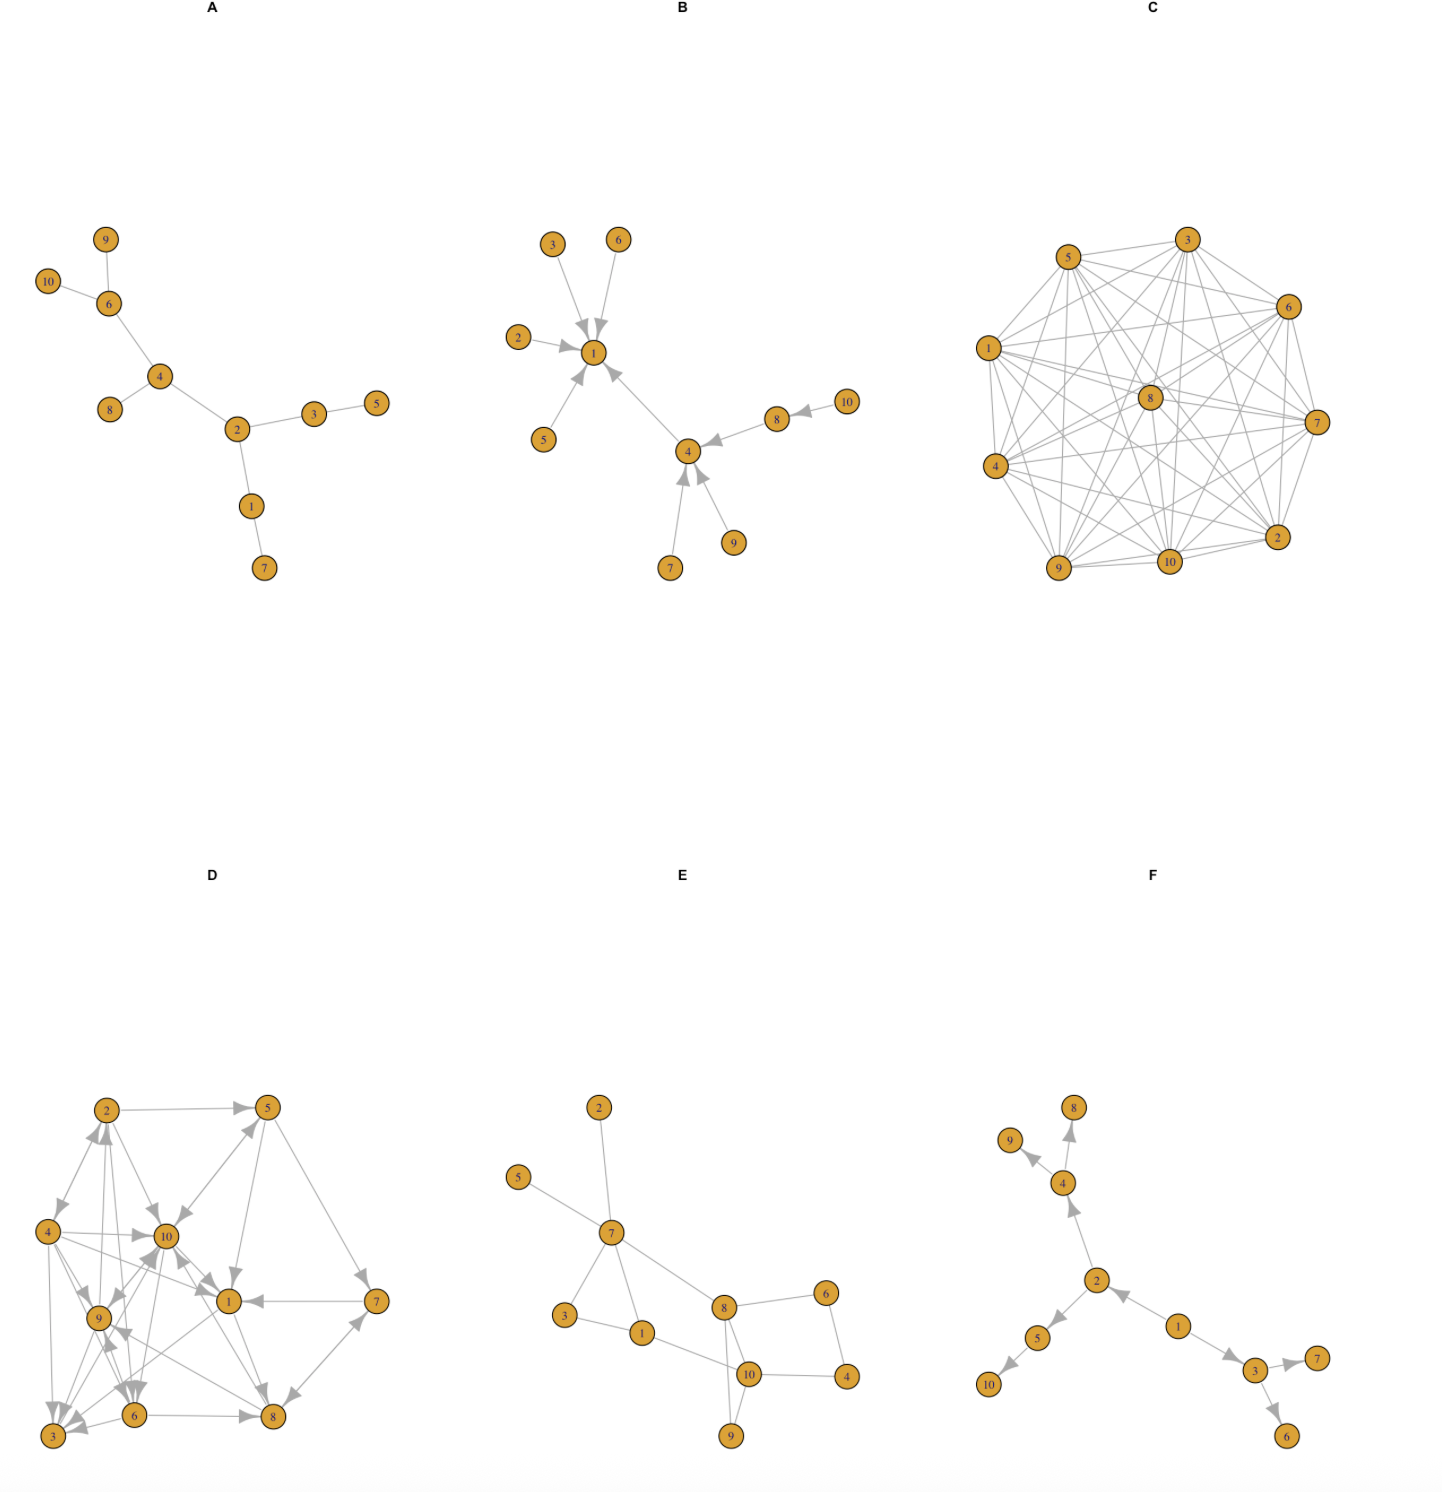
\includegraphics[width=20cm,height=20cm]{Imagenes/Redes.png}

\begin{itemize}
\tightlist
\item
  Número de conexiones
\item
  Número de nodos
\item
  Degree
\item
  Average degree
\item
  Degree distribution
\item
  Density
\item
  Adjacency matrix
\item
  Matriz de distancia
\item
  Diámetro
\item
  Nodos más distantes
\item
  Coeficiente de clusterización
\end{itemize}

Después escribe código en R que genere las gráficas de las redes y que
calcule las propiedades anteriores para cada red.

\begin{Shaded}
\begin{Highlighting}[]
\CommentTok{\# Generacion de redes}
\NormalTok{redA }\OtherTok{\textless{}{-}} \FunctionTok{make\_empty\_graph}\NormalTok{(}\DecValTok{10}\NormalTok{, }\ConstantTok{FALSE}\NormalTok{)}
\NormalTok{redA }\OtherTok{\textless{}{-}} \FunctionTok{add\_edges}\NormalTok{(redA, }\FunctionTok{c}\NormalTok{(}\DecValTok{10}\NormalTok{,}\DecValTok{6}\NormalTok{, }\DecValTok{9}\NormalTok{,}\DecValTok{6}\NormalTok{, }\DecValTok{6}\NormalTok{,}\DecValTok{4}\NormalTok{, }\DecValTok{8}\NormalTok{,}\DecValTok{4}\NormalTok{, }\DecValTok{4}\NormalTok{,}\DecValTok{2}\NormalTok{, }\DecValTok{2}\NormalTok{,}\DecValTok{3}\NormalTok{, }\DecValTok{3}\NormalTok{,}\DecValTok{5}\NormalTok{, }\DecValTok{2}\NormalTok{,}\DecValTok{1}\NormalTok{, }\DecValTok{1}\NormalTok{,}\DecValTok{7}\NormalTok{))}

\NormalTok{redB }\OtherTok{\textless{}{-}} \FunctionTok{make\_empty\_graph}\NormalTok{(}\DecValTok{10}\NormalTok{, }\ConstantTok{TRUE}\NormalTok{)}
\NormalTok{redB }\OtherTok{\textless{}{-}} \FunctionTok{add\_edges}\NormalTok{(redB, }\FunctionTok{c}\NormalTok{(}\DecValTok{2}\NormalTok{,}\DecValTok{1}\NormalTok{, }\DecValTok{3}\NormalTok{,}\DecValTok{1}\NormalTok{, }\DecValTok{6}\NormalTok{,}\DecValTok{1}\NormalTok{, }\DecValTok{5}\NormalTok{,}\DecValTok{1}\NormalTok{, }\DecValTok{4}\NormalTok{,}\DecValTok{1}\NormalTok{, }\DecValTok{10}\NormalTok{,}\DecValTok{8}\NormalTok{, }\DecValTok{8}\NormalTok{,}\DecValTok{4}\NormalTok{, }\DecValTok{9}\NormalTok{,}\DecValTok{4}\NormalTok{, }\DecValTok{7}\NormalTok{,}\DecValTok{4}\NormalTok{))}

\NormalTok{redC }\OtherTok{\textless{}{-}} \FunctionTok{make\_full\_graph}\NormalTok{(}\DecValTok{10}\NormalTok{, }\ConstantTok{FALSE}\NormalTok{)}

\NormalTok{redD }\OtherTok{\textless{}{-}} \FunctionTok{make\_empty\_graph}\NormalTok{(}\DecValTok{10}\NormalTok{, }\ConstantTok{TRUE}\NormalTok{)}
\NormalTok{redD }\OtherTok{\textless{}{-}} \FunctionTok{add\_edges}\NormalTok{(redD, }\FunctionTok{c}\NormalTok{(}\DecValTok{1}\NormalTok{,}\DecValTok{3}\NormalTok{, }\DecValTok{1}\NormalTok{,}\DecValTok{8}\NormalTok{, }\DecValTok{2}\NormalTok{,}\DecValTok{4}\NormalTok{, }\DecValTok{2}\NormalTok{,}\DecValTok{6}\NormalTok{, }\DecValTok{2}\NormalTok{,}\DecValTok{10}\NormalTok{, }\DecValTok{2}\NormalTok{,}\DecValTok{5}\NormalTok{, }\DecValTok{3}\NormalTok{,}\DecValTok{10}\NormalTok{, }\DecValTok{4}\NormalTok{,}\DecValTok{2}\NormalTok{, }\DecValTok{4}\NormalTok{,}\DecValTok{3}\NormalTok{, }\DecValTok{4}\NormalTok{,}\DecValTok{6}\NormalTok{, }\DecValTok{4}\NormalTok{,}\DecValTok{9}\NormalTok{, }\DecValTok{4}\NormalTok{,}\DecValTok{10}\NormalTok{, }\DecValTok{4}\NormalTok{,}\DecValTok{1}\NormalTok{, }\DecValTok{5}\NormalTok{,}\DecValTok{10}\NormalTok{, }\DecValTok{5}\NormalTok{,}\DecValTok{1}\NormalTok{, }\DecValTok{5}\NormalTok{,}\DecValTok{7}\NormalTok{, }\DecValTok{6}\NormalTok{,}\DecValTok{9}\NormalTok{, }\DecValTok{6}\NormalTok{,}\DecValTok{3}\NormalTok{, }\DecValTok{6}\NormalTok{,}\DecValTok{8}\NormalTok{, }\DecValTok{7}\NormalTok{,}\DecValTok{8}\NormalTok{, }\DecValTok{7}\NormalTok{,}\DecValTok{1}\NormalTok{, }\DecValTok{8}\NormalTok{,}\DecValTok{7}\NormalTok{, }\DecValTok{8}\NormalTok{,}\DecValTok{9}\NormalTok{, }\DecValTok{8}\NormalTok{,}\DecValTok{10}\NormalTok{, }\DecValTok{9}\NormalTok{,}\DecValTok{3}\NormalTok{, }\DecValTok{9}\NormalTok{,}\DecValTok{10}\NormalTok{, }\DecValTok{9}\NormalTok{,}\DecValTok{2}\NormalTok{, }\DecValTok{10}\NormalTok{,}\DecValTok{9}\NormalTok{, }\DecValTok{10}\NormalTok{,}\DecValTok{6}\NormalTok{, }\DecValTok{10}\NormalTok{,}\DecValTok{1}\NormalTok{, }\DecValTok{10}\NormalTok{,}\DecValTok{5}\NormalTok{))}

\NormalTok{redE }\OtherTok{\textless{}{-}} \FunctionTok{make\_empty\_graph}\NormalTok{(}\DecValTok{10}\NormalTok{, }\ConstantTok{FALSE}\NormalTok{)}
\NormalTok{redE }\OtherTok{\textless{}{-}} \FunctionTok{add\_edges}\NormalTok{(redE, }\FunctionTok{c}\NormalTok{(}\DecValTok{5}\NormalTok{,}\DecValTok{7}\NormalTok{, }\DecValTok{2}\NormalTok{,}\DecValTok{7}\NormalTok{, }\DecValTok{3}\NormalTok{,}\DecValTok{7}\NormalTok{, }\DecValTok{1}\NormalTok{,}\DecValTok{7}\NormalTok{, }\DecValTok{8}\NormalTok{,}\DecValTok{7}\NormalTok{, }\DecValTok{1}\NormalTok{,}\DecValTok{3}\NormalTok{, }\DecValTok{6}\NormalTok{,}\DecValTok{8}\NormalTok{, }\DecValTok{10}\NormalTok{,}\DecValTok{8}\NormalTok{, }\DecValTok{10}\NormalTok{,}\DecValTok{1}\NormalTok{, }\DecValTok{6}\NormalTok{,}\DecValTok{4}\NormalTok{, }\DecValTok{4}\NormalTok{,}\DecValTok{10}\NormalTok{, }\DecValTok{9}\NormalTok{,}\DecValTok{10}\NormalTok{, }\DecValTok{9}\NormalTok{,}\DecValTok{8}\NormalTok{))}

\NormalTok{redF }\OtherTok{\textless{}{-}} \FunctionTok{make\_empty\_graph}\NormalTok{(}\DecValTok{10}\NormalTok{, }\ConstantTok{TRUE}\NormalTok{)}
\NormalTok{redF }\OtherTok{\textless{}{-}} \FunctionTok{add\_edges}\NormalTok{(redF, }\FunctionTok{c}\NormalTok{(}\DecValTok{4}\NormalTok{,}\DecValTok{9}\NormalTok{, }\DecValTok{4}\NormalTok{,}\DecValTok{8}\NormalTok{, }\DecValTok{2}\NormalTok{,}\DecValTok{4}\NormalTok{, }\DecValTok{2}\NormalTok{,}\DecValTok{5}\NormalTok{, }\DecValTok{5}\NormalTok{,}\DecValTok{10}\NormalTok{, }\DecValTok{1}\NormalTok{,}\DecValTok{2}\NormalTok{, }\DecValTok{1}\NormalTok{,}\DecValTok{3}\NormalTok{, }\DecValTok{3}\NormalTok{,}\DecValTok{6}\NormalTok{, }\DecValTok{3}\NormalTok{,}\DecValTok{7}\NormalTok{))}

\CommentTok{\# Lista de las redes}
\NormalTok{redes\_AF }\OtherTok{\textless{}{-}} \FunctionTok{list}\NormalTok{(}\AttributeTok{redA=}\NormalTok{redA, }\AttributeTok{redB=}\NormalTok{redB, }\AttributeTok{redC=}\NormalTok{redC, }\AttributeTok{redD=}\NormalTok{redD, }\AttributeTok{redE=}\NormalTok{redE, }\AttributeTok{redF=}\NormalTok{redF)}

\CommentTok{\# Evaluacion de cada red}

\ControlFlowTok{for}\NormalTok{ (name }\ControlFlowTok{in} \FunctionTok{names}\NormalTok{(redes\_AF)) \{}
  
  \FunctionTok{cat}\NormalTok{(}\StringTok{"}\SpecialCharTok{\textbackslash{}n}\StringTok{Imagen de la"}\NormalTok{, name, }\StringTok{"}\SpecialCharTok{\textbackslash{}n}\StringTok{"}\NormalTok{)}
\NormalTok{  red }\OtherTok{\textless{}{-}}\NormalTok{ redes\_AF[[name]]}
  \FunctionTok{plot}\NormalTok{(red, }\AttributeTok{main=}\NormalTok{ name)}
  
  \FunctionTok{cat}\NormalTok{(}\StringTok{"}\SpecialCharTok{\textbackslash{}n}\StringTok{Número de conexiones:"}\NormalTok{, }\FunctionTok{gsize}\NormalTok{(red), }\StringTok{"}\SpecialCharTok{\textbackslash{}n}\StringTok{"}\NormalTok{) }
  \FunctionTok{cat}\NormalTok{(}\StringTok{"}\SpecialCharTok{\textbackslash{}n}\StringTok{Número de nodos:"}\NormalTok{, }\FunctionTok{gorder}\NormalTok{(red), }\StringTok{"}\SpecialCharTok{\textbackslash{}n}\StringTok{"}\NormalTok{)}
  \FunctionTok{cat}\NormalTok{(}\StringTok{"}\SpecialCharTok{\textbackslash{}n}\StringTok{Degree local:"}\NormalTok{, }\FunctionTok{degree}\NormalTok{(red, }\AttributeTok{mode =} \StringTok{"total"}\NormalTok{), }\StringTok{"}\SpecialCharTok{\textbackslash{}n}\StringTok{"}\NormalTok{) }
  \FunctionTok{cat}\NormalTok{(}\StringTok{"}\SpecialCharTok{\textbackslash{}n}\StringTok{Promedio del degree:"}\NormalTok{, }\FunctionTok{mean}\NormalTok{(}\FunctionTok{degree}\NormalTok{(red, }\AttributeTok{mode =} \StringTok{"total"}\NormalTok{)), }\StringTok{"}\SpecialCharTok{\textbackslash{}n}\StringTok{"}\NormalTok{)}
  
  \CommentTok{\# Degree distribution}
\NormalTok{  dd }\OtherTok{\textless{}{-}} \FunctionTok{degree\_distribution}\NormalTok{(red)}
  \FunctionTok{barplot}\NormalTok{(dd, }\AttributeTok{main=}\StringTok{\textquotesingle{}Distribucion del degree\textquotesingle{}}\NormalTok{, }\AttributeTok{ylim =} \FunctionTok{c}\NormalTok{(}\DecValTok{0}\SpecialCharTok{:}\DecValTok{1}\NormalTok{), }\AttributeTok{col=}\StringTok{\textquotesingle{}red\textquotesingle{}}\NormalTok{, }\AttributeTok{ylab =} \StringTok{"Pk"}\NormalTok{, }\AttributeTok{xlab =} \StringTok{"K"}\NormalTok{)}
  
  \FunctionTok{cat}\NormalTok{(}\StringTok{"}\SpecialCharTok{\textbackslash{}n}\StringTok{Densidad:"}\NormalTok{, }\FunctionTok{edge\_density}\NormalTok{(red), }\StringTok{"}\SpecialCharTok{\textbackslash{}n}\StringTok{"}\NormalTok{)}
  
  \FunctionTok{cat}\NormalTok{(}\StringTok{"}\SpecialCharTok{\textbackslash{}n}\StringTok{Matriz de adyacencia de la"}\NormalTok{, name, }\StringTok{"}\SpecialCharTok{\textbackslash{}n}\StringTok{"}\NormalTok{)}
  \FunctionTok{print}\NormalTok{(}\FunctionTok{as\_adjacency\_matrix}\NormalTok{(red))}
  
  \FunctionTok{cat}\NormalTok{(}\StringTok{"}\SpecialCharTok{\textbackslash{}n}\StringTok{Matriz de distancias de la"}\NormalTok{, name, }\StringTok{"}\SpecialCharTok{\textbackslash{}n}\StringTok{"}\NormalTok{)}
  \FunctionTok{print}\NormalTok{(}\FunctionTok{distances}\NormalTok{(red))}
  
  \FunctionTok{cat}\NormalTok{(}\StringTok{"}\SpecialCharTok{\textbackslash{}n}\StringTok{Diámetro:"}\NormalTok{, }\FunctionTok{diameter}\NormalTok{(red), }\StringTok{"}\SpecialCharTok{\textbackslash{}n}\StringTok{"}\NormalTok{) }
  \CommentTok{\# cat("\textbackslash{}n", name, "\textbackslash{}n") \# Nodos más distantes}
  \FunctionTok{cat}\NormalTok{(}\StringTok{"}\SpecialCharTok{\textbackslash{}n}\StringTok{Coeficiente de clusterización local:"}\NormalTok{, }\FunctionTok{transitivity}\NormalTok{(red, }\AttributeTok{type =} \StringTok{"local"}\NormalTok{), }\StringTok{"}\SpecialCharTok{\textbackslash{}n}\StringTok{"}\NormalTok{)}
  \FunctionTok{cat}\NormalTok{(}\StringTok{"}\SpecialCharTok{\textbackslash{}n}\StringTok{Coeficiente de clusterización"}\NormalTok{, }\FunctionTok{transitivity}\NormalTok{(red, }\AttributeTok{type =} \StringTok{"global"}\NormalTok{ ), }\StringTok{"}\SpecialCharTok{\textbackslash{}n}\StringTok{"}\NormalTok{)}
  
\NormalTok{\}}
\end{Highlighting}
\end{Shaded}

\begin{verbatim}
## 
## Imagen de la redA
\end{verbatim}

\includegraphics{GF_Tarea_04_2025_files/figure-latex/unnamed-chunk-9-1.pdf}

\begin{verbatim}
## 
## Número de conexiones: 9 
## 
## Número de nodos: 10 
## 
## Degree local: 2 3 2 3 1 3 1 1 1 1 
## 
## Promedio del degree: 1.8
\end{verbatim}

\includegraphics{GF_Tarea_04_2025_files/figure-latex/unnamed-chunk-9-2.pdf}

\begin{verbatim}
## 
## Densidad: 0.2 
## 
## Matriz de adyacencia de la redA 
## 10 x 10 sparse Matrix of class "dgCMatrix"
##                          
##  [1,] . 1 . . . . 1 . . .
##  [2,] 1 . 1 1 . . . . . .
##  [3,] . 1 . . 1 . . . . .
##  [4,] . 1 . . . 1 . 1 . .
##  [5,] . . 1 . . . . . . .
##  [6,] . . . 1 . . . . 1 1
##  [7,] 1 . . . . . . . . .
##  [8,] . . . 1 . . . . . .
##  [9,] . . . . . 1 . . . .
## [10,] . . . . . 1 . . . .
## 
## Matriz de distancias de la redA 
##       [,1] [,2] [,3] [,4] [,5] [,6] [,7] [,8] [,9] [,10]
##  [1,]    0    1    2    2    3    3    1    3    4     4
##  [2,]    1    0    1    1    2    2    2    2    3     3
##  [3,]    2    1    0    2    1    3    3    3    4     4
##  [4,]    2    1    2    0    3    1    3    1    2     2
##  [5,]    3    2    1    3    0    4    4    4    5     5
##  [6,]    3    2    3    1    4    0    4    2    1     1
##  [7,]    1    2    3    3    4    4    0    4    5     5
##  [8,]    3    2    3    1    4    2    4    0    3     3
##  [9,]    4    3    4    2    5    1    5    3    0     2
## [10,]    4    3    4    2    5    1    5    3    2     0
## 
## Diámetro: 5 
## 
## Coeficiente de clusterización local: 0 0 0 0 NaN 0 NaN NaN NaN NaN 
## 
## Coeficiente de clusterización 0 
## 
## Imagen de la redB
\end{verbatim}

\includegraphics{GF_Tarea_04_2025_files/figure-latex/unnamed-chunk-9-3.pdf}

\begin{verbatim}
## 
## Número de conexiones: 9 
## 
## Número de nodos: 10 
## 
## Degree local: 5 1 1 4 1 1 1 2 1 1 
## 
## Promedio del degree: 1.8
\end{verbatim}

\includegraphics{GF_Tarea_04_2025_files/figure-latex/unnamed-chunk-9-4.pdf}

\begin{verbatim}
## 
## Densidad: 0.1 
## 
## Matriz de adyacencia de la redB 
## 10 x 10 sparse Matrix of class "dgCMatrix"
##                          
##  [1,] . . . . . . . . . .
##  [2,] 1 . . . . . . . . .
##  [3,] 1 . . . . . . . . .
##  [4,] 1 . . . . . . . . .
##  [5,] 1 . . . . . . . . .
##  [6,] 1 . . . . . . . . .
##  [7,] . . . 1 . . . . . .
##  [8,] . . . 1 . . . . . .
##  [9,] . . . 1 . . . . . .
## [10,] . . . . . . . 1 . .
## 
## Matriz de distancias de la redB 
##       [,1] [,2] [,3] [,4] [,5] [,6] [,7] [,8] [,9] [,10]
##  [1,]    0    1    1    1    1    1    2    2    2     3
##  [2,]    1    0    2    2    2    2    3    3    3     4
##  [3,]    1    2    0    2    2    2    3    3    3     4
##  [4,]    1    2    2    0    2    2    1    1    1     2
##  [5,]    1    2    2    2    0    2    3    3    3     4
##  [6,]    1    2    2    2    2    0    3    3    3     4
##  [7,]    2    3    3    1    3    3    0    2    2     3
##  [8,]    2    3    3    1    3    3    2    0    2     1
##  [9,]    2    3    3    1    3    3    2    2    0     3
## [10,]    3    4    4    2    4    4    3    1    3     0
## 
## Diámetro: 3 
## 
## Coeficiente de clusterización local: 0 NaN NaN 0 NaN NaN NaN 0 NaN NaN 
## 
## Coeficiente de clusterización 0 
## 
## Imagen de la redC
\end{verbatim}

\includegraphics{GF_Tarea_04_2025_files/figure-latex/unnamed-chunk-9-5.pdf}

\begin{verbatim}
## 
## Número de conexiones: 45 
## 
## Número de nodos: 10 
## 
## Degree local: 9 9 9 9 9 9 9 9 9 9 
## 
## Promedio del degree: 9
\end{verbatim}

\includegraphics{GF_Tarea_04_2025_files/figure-latex/unnamed-chunk-9-6.pdf}

\begin{verbatim}
## 
## Densidad: 1 
## 
## Matriz de adyacencia de la redC 
## 10 x 10 sparse Matrix of class "dgCMatrix"
##                          
##  [1,] . 1 1 1 1 1 1 1 1 1
##  [2,] 1 . 1 1 1 1 1 1 1 1
##  [3,] 1 1 . 1 1 1 1 1 1 1
##  [4,] 1 1 1 . 1 1 1 1 1 1
##  [5,] 1 1 1 1 . 1 1 1 1 1
##  [6,] 1 1 1 1 1 . 1 1 1 1
##  [7,] 1 1 1 1 1 1 . 1 1 1
##  [8,] 1 1 1 1 1 1 1 . 1 1
##  [9,] 1 1 1 1 1 1 1 1 . 1
## [10,] 1 1 1 1 1 1 1 1 1 .
## 
## Matriz de distancias de la redC 
##       [,1] [,2] [,3] [,4] [,5] [,6] [,7] [,8] [,9] [,10]
##  [1,]    0    1    1    1    1    1    1    1    1     1
##  [2,]    1    0    1    1    1    1    1    1    1     1
##  [3,]    1    1    0    1    1    1    1    1    1     1
##  [4,]    1    1    1    0    1    1    1    1    1     1
##  [5,]    1    1    1    1    0    1    1    1    1     1
##  [6,]    1    1    1    1    1    0    1    1    1     1
##  [7,]    1    1    1    1    1    1    0    1    1     1
##  [8,]    1    1    1    1    1    1    1    0    1     1
##  [9,]    1    1    1    1    1    1    1    1    0     1
## [10,]    1    1    1    1    1    1    1    1    1     0
## 
## Diámetro: 1 
## 
## Coeficiente de clusterización local: 1 1 1 1 1 1 1 1 1 1 
## 
## Coeficiente de clusterización 1 
## 
## Imagen de la redD
\end{verbatim}

\includegraphics{GF_Tarea_04_2025_files/figure-latex/unnamed-chunk-9-7.pdf}

\begin{verbatim}
## 
## Número de conexiones: 31 
## 
## Número de nodos: 10 
## 
## Degree local: 6 6 5 7 5 6 4 6 7 10 
## 
## Promedio del degree: 6.2
\end{verbatim}

\includegraphics{GF_Tarea_04_2025_files/figure-latex/unnamed-chunk-9-8.pdf}

\begin{verbatim}
## 
## Densidad: 0.3444444 
## 
## Matriz de adyacencia de la redD 
## 10 x 10 sparse Matrix of class "dgCMatrix"
##                          
##  [1,] . . 1 . . . . 1 . .
##  [2,] . . . 1 1 1 . . . 1
##  [3,] . . . . . . . . . 1
##  [4,] 1 1 1 . . 1 . . 1 1
##  [5,] 1 . . . . . 1 . . 1
##  [6,] . . 1 . . . . 1 1 .
##  [7,] 1 . . . . . . 1 . .
##  [8,] . . . . . . 1 . 1 1
##  [9,] . 1 1 . . . . . . 1
## [10,] 1 . . . 1 1 . . 1 .
## 
## Matriz de distancias de la redD 
##       [,1] [,2] [,3] [,4] [,5] [,6] [,7] [,8] [,9] [,10]
##  [1,]    0    2    1    1    1    2    1    1    2     1
##  [2,]    2    0    2    1    1    1    2    2    1     1
##  [3,]    1    2    0    1    2    1    2    2    1     1
##  [4,]    1    1    1    0    2    1    2    2    1     1
##  [5,]    1    1    2    2    0    2    1    2    2     1
##  [6,]    2    1    1    1    2    0    2    1    1     1
##  [7,]    1    2    2    2    1    2    0    1    2     2
##  [8,]    1    2    2    2    2    1    1    0    1     1
##  [9,]    2    1    1    1    2    1    2    1    0     1
## [10,]    1    1    1    1    1    1    2    1    1     0
## 
## Diámetro: 4 
## 
## Coeficiente de clusterización local: 0.4666667 0.7 0.8 0.7333333 0.5 0.7333333 0.6666667 0.5 0.7333333 0.5714286 
## 
## Coeficiente de clusterización 0.6377953 
## 
## Imagen de la redE
\end{verbatim}

\includegraphics{GF_Tarea_04_2025_files/figure-latex/unnamed-chunk-9-9.pdf}

\begin{verbatim}
## 
## Número de conexiones: 13 
## 
## Número de nodos: 10 
## 
## Degree local: 3 1 2 2 1 2 5 4 2 4 
## 
## Promedio del degree: 2.6
\end{verbatim}

\includegraphics{GF_Tarea_04_2025_files/figure-latex/unnamed-chunk-9-10.pdf}

\begin{verbatim}
## 
## Densidad: 0.2888889 
## 
## Matriz de adyacencia de la redE 
## 10 x 10 sparse Matrix of class "dgCMatrix"
##                          
##  [1,] . . 1 . . . 1 . . 1
##  [2,] . . . . . . 1 . . .
##  [3,] 1 . . . . . 1 . . .
##  [4,] . . . . . 1 . . . 1
##  [5,] . . . . . . 1 . . .
##  [6,] . . . 1 . . . 1 . .
##  [7,] 1 1 1 . 1 . . 1 . .
##  [8,] . . . . . 1 1 . 1 1
##  [9,] . . . . . . . 1 . 1
## [10,] 1 . . 1 . . . 1 1 .
## 
## Matriz de distancias de la redE 
##       [,1] [,2] [,3] [,4] [,5] [,6] [,7] [,8] [,9] [,10]
##  [1,]    0    2    1    2    2    3    1    2    2     1
##  [2,]    2    0    2    4    2    3    1    2    3     3
##  [3,]    1    2    0    3    2    3    1    2    3     2
##  [4,]    2    4    3    0    4    1    3    2    2     1
##  [5,]    2    2    2    4    0    3    1    2    3     3
##  [6,]    3    3    3    1    3    0    2    1    2     2
##  [7,]    1    1    1    3    1    2    0    1    2     2
##  [8,]    2    2    2    2    2    1    1    0    1     1
##  [9,]    2    3    3    2    3    2    2    1    0     1
## [10,]    1    3    2    1    3    2    2    1    1     0
## 
## Diámetro: 4 
## 
## Coeficiente de clusterización local: 0.3333333 NaN 1 0 NaN 0 0.1 0.1666667 1 0.1666667 
## 
## Coeficiente de clusterización 0.2068966 
## 
## Imagen de la redF
\end{verbatim}

\includegraphics{GF_Tarea_04_2025_files/figure-latex/unnamed-chunk-9-11.pdf}

\begin{verbatim}
## 
## Número de conexiones: 9 
## 
## Número de nodos: 10 
## 
## Degree local: 2 3 3 3 2 1 1 1 1 1 
## 
## Promedio del degree: 1.8
\end{verbatim}

\includegraphics{GF_Tarea_04_2025_files/figure-latex/unnamed-chunk-9-12.pdf}

\begin{verbatim}
## 
## Densidad: 0.1 
## 
## Matriz de adyacencia de la redF 
## 10 x 10 sparse Matrix of class "dgCMatrix"
##                          
##  [1,] . 1 1 . . . . . . .
##  [2,] . . . 1 1 . . . . .
##  [3,] . . . . . 1 1 . . .
##  [4,] . . . . . . . 1 1 .
##  [5,] . . . . . . . . . 1
##  [6,] . . . . . . . . . .
##  [7,] . . . . . . . . . .
##  [8,] . . . . . . . . . .
##  [9,] . . . . . . . . . .
## [10,] . . . . . . . . . .
## 
## Matriz de distancias de la redF 
##       [,1] [,2] [,3] [,4] [,5] [,6] [,7] [,8] [,9] [,10]
##  [1,]    0    1    1    2    2    2    2    3    3     3
##  [2,]    1    0    2    1    1    3    3    2    2     2
##  [3,]    1    2    0    3    3    1    1    4    4     4
##  [4,]    2    1    3    0    2    4    4    1    1     3
##  [5,]    2    1    3    2    0    4    4    3    3     1
##  [6,]    2    3    1    4    4    0    2    5    5     5
##  [7,]    2    3    1    4    4    2    0    5    5     5
##  [8,]    3    2    4    1    3    5    5    0    2     4
##  [9,]    3    2    4    1    3    5    5    2    0     4
## [10,]    3    2    4    3    1    5    5    4    4     0
## 
## Diámetro: 3 
## 
## Coeficiente de clusterización local: 0 0 0 0 0 NaN NaN NaN NaN NaN 
## 
## Coeficiente de clusterización 0
\end{verbatim}

\begin{enumerate}
\def\labelenumi{\arabic{enumi}.}
\tightlist
\item
  \textbf{Karate}
\end{enumerate}

Considera la red del club de Karate de Zachary.
\href{https://en.wikipedia.org/wiki/Zachary\%27s_karate_club}{Acá}
puedes leer sobre eso. En igraph la gráfica está precargada

\begin{Shaded}
\begin{Highlighting}[]
\NormalTok{karate }\OtherTok{\textless{}{-}} \FunctionTok{make\_graph}\NormalTok{(}\StringTok{"Zachary"}\NormalTok{)}
\FunctionTok{plot}\NormalTok{(karate)}
\end{Highlighting}
\end{Shaded}

\includegraphics{GF_Tarea_04_2025_files/figure-latex/unnamed-chunk-10-1.pdf}

\begin{itemize}
\tightlist
\item
  ¿Cuántos nodos y conexiones tiene?
\item
  ¿Quiénes son los nodos y cuál es la regla de conexión?
\item
  ¿Qué tan densa es la red?
\item
  ¿Cómo obtienes la matriz de adyacencia?
\item
  ¿Es una red dirigida, pesada?
\item
  Calcula y gráfica la distribución de conectividades
\item
  Calcula el diámetro, la matriz de distancias y la distancia promedio
\item
  Encuentra la trayectoria de los nodos más alejados.
\item
  Existen nodos con coefeiciente de clusterización 1. ¿Qué significa?
\item
  Mide, con al menos tres medidas de centralidad, los nodos más
  importantes.
\end{itemize}

\begin{Shaded}
\begin{Highlighting}[]
\FunctionTok{cat}\NormalTok{(}\StringTok{"}\SpecialCharTok{\textbackslash{}n}\StringTok{Número de conexiones:"}\NormalTok{, }\FunctionTok{gsize}\NormalTok{(karate), }\StringTok{"}\SpecialCharTok{\textbackslash{}n}\StringTok{"}\NormalTok{) }
\end{Highlighting}
\end{Shaded}

\begin{verbatim}
## 
## Número de conexiones: 78
\end{verbatim}

\begin{Shaded}
\begin{Highlighting}[]
\FunctionTok{cat}\NormalTok{(}\StringTok{"}\SpecialCharTok{\textbackslash{}n}\StringTok{Número de nodos:"}\NormalTok{, }\FunctionTok{gorder}\NormalTok{(karate), }\StringTok{"}\SpecialCharTok{\textbackslash{}n}\StringTok{"}\NormalTok{)}
\end{Highlighting}
\end{Shaded}

\begin{verbatim}
## 
## Número de nodos: 34
\end{verbatim}

\begin{Shaded}
\begin{Highlighting}[]
\CommentTok{\# ¿Quiénes son los nodos y cuál es la regla de conexión?}
\FunctionTok{cat}\NormalTok{(}\StringTok{"}\SpecialCharTok{\textbackslash{}n}\StringTok{Densidad:"}\NormalTok{, }\FunctionTok{edge\_density}\NormalTok{(karate), }\StringTok{"}\SpecialCharTok{\textbackslash{}n}\StringTok{"}\NormalTok{)}
\end{Highlighting}
\end{Shaded}

\begin{verbatim}
## 
## Densidad: 0.1390374
\end{verbatim}

\begin{Shaded}
\begin{Highlighting}[]
\FunctionTok{cat}\NormalTok{(}\StringTok{"}\SpecialCharTok{\textbackslash{}n}\StringTok{Matriz de adyacencia"}\NormalTok{, }\StringTok{"}\SpecialCharTok{\textbackslash{}n}\StringTok{"}\NormalTok{)}
\end{Highlighting}
\end{Shaded}

\begin{verbatim}
## 
## Matriz de adyacencia
\end{verbatim}

\begin{Shaded}
\begin{Highlighting}[]
\FunctionTok{print}\NormalTok{(}\FunctionTok{as\_adjacency\_matrix}\NormalTok{(karate))}
\end{Highlighting}
\end{Shaded}

\begin{verbatim}
## 34 x 34 sparse Matrix of class "dgCMatrix"
##                                                                          
##  [1,] . 1 1 1 1 1 1 1 1 . 1 1 1 1 . . . 1 . 1 . 1 . . . . . . . . . 1 . .
##  [2,] 1 . 1 1 . . . 1 . . . . . 1 . . . 1 . 1 . 1 . . . . . . . . 1 . . .
##  [3,] 1 1 . 1 . . . 1 1 1 . . . 1 . . . . . . . . . . . . . 1 1 . . . 1 .
##  [4,] 1 1 1 . . . . 1 . . . . 1 1 . . . . . . . . . . . . . . . . . . . .
##  [5,] 1 . . . . . 1 . . . 1 . . . . . . . . . . . . . . . . . . . . . . .
##  [6,] 1 . . . . . 1 . . . 1 . . . . . 1 . . . . . . . . . . . . . . . . .
##  [7,] 1 . . . 1 1 . . . . . . . . . . 1 . . . . . . . . . . . . . . . . .
##  [8,] 1 1 1 1 . . . . . . . . . . . . . . . . . . . . . . . . . . . . . .
##  [9,] 1 . 1 . . . . . . . . . . . . . . . . . . . . . . . . . . . 1 . 1 1
## [10,] . . 1 . . . . . . . . . . . . . . . . . . . . . . . . . . . . . . 1
## [11,] 1 . . . 1 1 . . . . . . . . . . . . . . . . . . . . . . . . . . . .
## [12,] 1 . . . . . . . . . . . . . . . . . . . . . . . . . . . . . . . . .
## [13,] 1 . . 1 . . . . . . . . . . . . . . . . . . . . . . . . . . . . . .
## [14,] 1 1 1 1 . . . . . . . . . . . . . . . . . . . . . . . . . . . . . 1
## [15,] . . . . . . . . . . . . . . . . . . . . . . . . . . . . . . . . 1 1
## [16,] . . . . . . . . . . . . . . . . . . . . . . . . . . . . . . . . 1 1
## [17,] . . . . . 1 1 . . . . . . . . . . . . . . . . . . . . . . . . . . .
## [18,] 1 1 . . . . . . . . . . . . . . . . . . . . . . . . . . . . . . . .
## [19,] . . . . . . . . . . . . . . . . . . . . . . . . . . . . . . . . 1 1
## [20,] 1 1 . . . . . . . . . . . . . . . . . . . . . . . . . . . . . . . 1
## [21,] . . . . . . . . . . . . . . . . . . . . . . . . . . . . . . . . 1 1
## [22,] 1 1 . . . . . . . . . . . . . . . . . . . . . . . . . . . . . . . .
## [23,] . . . . . . . . . . . . . . . . . . . . . . . . . . . . . . . . 1 1
## [24,] . . . . . . . . . . . . . . . . . . . . . . . . . 1 . 1 . 1 . . 1 1
## [25,] . . . . . . . . . . . . . . . . . . . . . . . . . 1 . 1 . . . 1 . .
## [26,] . . . . . . . . . . . . . . . . . . . . . . . 1 1 . . . . . . 1 . .
## [27,] . . . . . . . . . . . . . . . . . . . . . . . . . . . . . 1 . . . 1
## [28,] . . 1 . . . . . . . . . . . . . . . . . . . . 1 1 . . . . . . . . 1
## [29,] . . 1 . . . . . . . . . . . . . . . . . . . . . . . . . . . . 1 . 1
## [30,] . . . . . . . . . . . . . . . . . . . . . . . 1 . . 1 . . . . . 1 1
## [31,] . 1 . . . . . . 1 . . . . . . . . . . . . . . . . . . . . . . . 1 1
## [32,] 1 . . . . . . . . . . . . . . . . . . . . . . . 1 1 . . 1 . . . 1 1
## [33,] . . 1 . . . . . 1 . . . . . 1 1 . . 1 . 1 . 1 1 . . . . . 1 1 1 . 1
## [34,] . . . . . . . . 1 1 . . . 1 1 1 . . 1 1 1 . 1 1 . . 1 1 1 1 1 1 1 .
\end{verbatim}

\begin{Shaded}
\begin{Highlighting}[]
\FunctionTok{cat}\NormalTok{(}\StringTok{"}\SpecialCharTok{\textbackslash{}n}\StringTok{Calculo y grafico del degree"}\NormalTok{, }\StringTok{"}\SpecialCharTok{\textbackslash{}n}\StringTok{"}\NormalTok{)}
\end{Highlighting}
\end{Shaded}

\begin{verbatim}
## 
## Calculo y grafico del degree
\end{verbatim}

\begin{Shaded}
\begin{Highlighting}[]
\NormalTok{dd }\OtherTok{\textless{}{-}} \FunctionTok{degree\_distribution}\NormalTok{(karate)}
\FunctionTok{barplot}\NormalTok{(dd, }\AttributeTok{main=}\StringTok{\textquotesingle{}Distribucion del degree\textquotesingle{}}\NormalTok{, }\AttributeTok{ylim =} \FunctionTok{c}\NormalTok{(}\DecValTok{0}\SpecialCharTok{:}\DecValTok{1}\NormalTok{), }\AttributeTok{col=}\StringTok{\textquotesingle{}red\textquotesingle{}}\NormalTok{, }\AttributeTok{ylab =} \StringTok{"Pk"}\NormalTok{, }\AttributeTok{xlab =} \StringTok{"K"}\NormalTok{)}
\end{Highlighting}
\end{Shaded}

\includegraphics{GF_Tarea_04_2025_files/figure-latex/unnamed-chunk-11-1.pdf}

\begin{Shaded}
\begin{Highlighting}[]
\FunctionTok{cat}\NormalTok{(}\StringTok{"}\SpecialCharTok{\textbackslash{}n}\StringTok{Diámetro:"}\NormalTok{, }\FunctionTok{diameter}\NormalTok{(karate), }\StringTok{"}\SpecialCharTok{\textbackslash{}n}\StringTok{"}\NormalTok{)}
\end{Highlighting}
\end{Shaded}

\begin{verbatim}
## 
## Diámetro: 5
\end{verbatim}

\begin{Shaded}
\begin{Highlighting}[]
\FunctionTok{cat}\NormalTok{(}\StringTok{"}\SpecialCharTok{\textbackslash{}n}\StringTok{Matriz de distancias"}\NormalTok{, }\StringTok{"}\SpecialCharTok{\textbackslash{}n}\StringTok{"}\NormalTok{)}
\end{Highlighting}
\end{Shaded}

\begin{verbatim}
## 
## Matriz de distancias
\end{verbatim}

\begin{Shaded}
\begin{Highlighting}[]
\FunctionTok{print}\NormalTok{(}\FunctionTok{distances}\NormalTok{(karate))}
\end{Highlighting}
\end{Shaded}

\begin{verbatim}
##       [,1] [,2] [,3] [,4] [,5] [,6] [,7] [,8] [,9] [,10] [,11] [,12] [,13]
##  [1,]    0    1    1    1    1    1    1    1    1     2     1     1     1
##  [2,]    1    0    1    1    2    2    2    1    2     2     2     2     2
##  [3,]    1    1    0    1    2    2    2    1    1     1     2     2     2
##  [4,]    1    1    1    0    2    2    2    1    2     2     2     2     1
##  [5,]    1    2    2    2    0    2    1    2    2     3     1     2     2
##  [6,]    1    2    2    2    2    0    1    2    2     3     1     2     2
##  [7,]    1    2    2    2    1    1    0    2    2     3     2     2     2
##  [8,]    1    1    1    1    2    2    2    0    2     2     2     2     2
##  [9,]    1    2    1    2    2    2    2    2    0     2     2     2     2
## [10,]    2    2    1    2    3    3    3    2    2     0     3     3     3
## [11,]    1    2    2    2    1    1    2    2    2     3     0     2     2
## [12,]    1    2    2    2    2    2    2    2    2     3     2     0     2
## [13,]    1    2    2    1    2    2    2    2    2     3     2     2     0
## [14,]    1    1    1    1    2    2    2    2    2     2     2     2     2
## [15,]    3    3    2    3    4    4    4    3    2     2     4     4     4
## [16,]    3    3    2    3    4    4    4    3    2     2     4     4     4
## [17,]    2    3    3    3    2    1    1    3    3     4     2     3     3
## [18,]    1    1    2    2    2    2    2    2    2     3     2     2     2
## [19,]    3    3    2    3    4    4    4    3    2     2     4     4     4
## [20,]    1    1    2    2    2    2    2    2    2     2     2     2     2
## [21,]    3    3    2    3    4    4    4    3    2     2     4     4     4
## [22,]    1    1    2    2    2    2    2    2    2     3     2     2     2
## [23,]    3    3    2    3    4    4    4    3    2     2     4     4     4
## [24,]    3    3    2    3    4    4    4    3    2     2     4     4     4
## [25,]    2    3    2    3    3    3    3    3    3     3     3     3     3
## [26,]    2    3    3    3    3    3    3    3    3     3     3     3     3
## [27,]    3    3    3    3    4    4    4    4    2     2     4     4     4
## [28,]    2    2    1    2    3    3    3    2    2     2     3     3     3
## [29,]    2    2    1    2    3    3    3    2    2     2     3     3     3
## [30,]    3    3    2    3    4    4    4    3    2     2     4     4     4
## [31,]    2    1    2    2    3    3    3    2    1     2     3     3     3
## [32,]    1    2    2    2    2    2    2    2    2     2     2     2     2
## [33,]    2    2    1    2    3    3    3    2    1     2     3     3     3
## [34,]    2    2    2    2    3    3    3    3    1     1     3     3     3
##       [,14] [,15] [,16] [,17] [,18] [,19] [,20] [,21] [,22] [,23] [,24] [,25]
##  [1,]     1     3     3     2     1     3     1     3     1     3     3     2
##  [2,]     1     3     3     3     1     3     1     3     1     3     3     3
##  [3,]     1     2     2     3     2     2     2     2     2     2     2     2
##  [4,]     1     3     3     3     2     3     2     3     2     3     3     3
##  [5,]     2     4     4     2     2     4     2     4     2     4     4     3
##  [6,]     2     4     4     1     2     4     2     4     2     4     4     3
##  [7,]     2     4     4     1     2     4     2     4     2     4     4     3
##  [8,]     2     3     3     3     2     3     2     3     2     3     3     3
##  [9,]     2     2     2     3     2     2     2     2     2     2     2     3
## [10,]     2     2     2     4     3     2     2     2     3     2     2     3
## [11,]     2     4     4     2     2     4     2     4     2     4     4     3
## [12,]     2     4     4     3     2     4     2     4     2     4     4     3
## [13,]     2     4     4     3     2     4     2     4     2     4     4     3
## [14,]     0     2     2     3     2     2     2     2     2     2     2     3
## [15,]     2     0     2     5     4     2     2     2     4     2     2     3
## [16,]     2     2     0     5     4     2     2     2     4     2     2     3
## [17,]     3     5     5     0     3     5     3     5     3     5     5     4
## [18,]     2     4     4     3     0     4     2     4     2     4     4     3
## [19,]     2     2     2     5     4     0     2     2     4     2     2     3
## [20,]     2     2     2     3     2     2     0     2     2     2     2     3
## [21,]     2     2     2     5     4     2     2     0     4     2     2     3
## [22,]     2     4     4     3     2     4     2     4     0     4     4     3
## [23,]     2     2     2     5     4     2     2     2     4     0     2     3
## [24,]     2     2     2     5     4     2     2     2     4     2     0     2
## [25,]     3     3     3     4     3     3     3     3     3     3     2     0
## [26,]     3     3     3     4     3     3     3     3     3     3     1     1
## [27,]     2     2     2     5     4     2     2     2     4     2     2     3
## [28,]     2     2     2     4     3     2     2     2     3     2     1     1
## [29,]     2     2     2     4     3     2     2     2     3     2     2     2
## [30,]     2     2     2     5     4     2     2     2     4     2     1     3
## [31,]     2     2     2     4     2     2     2     2     2     2     2     3
## [32,]     2     2     2     3     2     2     2     2     2     2     2     1
## [33,]     2     1     1     4     3     1     2     1     3     1     1     2
## [34,]     1     1     1     4     3     1     1     1     3     1     1     2
##       [,26] [,27] [,28] [,29] [,30] [,31] [,32] [,33] [,34]
##  [1,]     2     3     2     2     3     2     1     2     2
##  [2,]     3     3     2     2     3     1     2     2     2
##  [3,]     3     3     1     1     2     2     2     1     2
##  [4,]     3     3     2     2     3     2     2     2     2
##  [5,]     3     4     3     3     4     3     2     3     3
##  [6,]     3     4     3     3     4     3     2     3     3
##  [7,]     3     4     3     3     4     3     2     3     3
##  [8,]     3     4     2     2     3     2     2     2     3
##  [9,]     3     2     2     2     2     1     2     1     1
## [10,]     3     2     2     2     2     2     2     2     1
## [11,]     3     4     3     3     4     3     2     3     3
## [12,]     3     4     3     3     4     3     2     3     3
## [13,]     3     4     3     3     4     3     2     3     3
## [14,]     3     2     2     2     2     2     2     2     1
## [15,]     3     2     2     2     2     2     2     1     1
## [16,]     3     2     2     2     2     2     2     1     1
## [17,]     4     5     4     4     5     4     3     4     4
## [18,]     3     4     3     3     4     2     2     3     3
## [19,]     3     2     2     2     2     2     2     1     1
## [20,]     3     2     2     2     2     2     2     2     1
## [21,]     3     2     2     2     2     2     2     1     1
## [22,]     3     4     3     3     4     2     2     3     3
## [23,]     3     2     2     2     2     2     2     1     1
## [24,]     1     2     1     2     1     2     2     1     1
## [25,]     1     3     1     2     3     3     1     2     2
## [26,]     0     3     2     2     2     3     1     2     2
## [27,]     3     0     2     2     1     2     2     2     1
## [28,]     2     2     0     2     2     2     2     2     1
## [29,]     2     2     2     0     2     2     1     2     1
## [30,]     2     1     2     2     0     2     2     1     1
## [31,]     3     2     2     2     2     0     2     1     1
## [32,]     1     2     2     1     2     2     0     1     1
## [33,]     2     2     2     2     1     1     1     0     1
## [34,]     2     1     1     1     1     1     1     1     0
\end{verbatim}

\begin{Shaded}
\begin{Highlighting}[]
\FunctionTok{cat}\NormalTok{(}\StringTok{"}\SpecialCharTok{\textbackslash{}n}\StringTok{Promedio de la distancia:"}\NormalTok{, }\FunctionTok{mean\_distance}\NormalTok{(karate), }\StringTok{"}\SpecialCharTok{\textbackslash{}n}\StringTok{"}\NormalTok{)}
\end{Highlighting}
\end{Shaded}

\begin{verbatim}
## 
## Promedio de la distancia: 2.4082
\end{verbatim}

\begin{Shaded}
\begin{Highlighting}[]
\FunctionTok{cat}\NormalTok{(}\StringTok{"}\SpecialCharTok{\textbackslash{}n}\StringTok{Trayectoria de los nodos mas alejados"}\NormalTok{, }\StringTok{"}\SpecialCharTok{\textbackslash{}n}\StringTok{"}\NormalTok{)}
\end{Highlighting}
\end{Shaded}

\begin{verbatim}
## 
## Trayectoria de los nodos mas alejados
\end{verbatim}

\begin{Shaded}
\begin{Highlighting}[]
\NormalTok{n\_lejanos }\OtherTok{\textless{}{-}} \FunctionTok{get\_diameter}\NormalTok{(karate)}
\NormalTok{n\_lejanos}
\end{Highlighting}
\end{Shaded}

\begin{verbatim}
## + 6/34 vertices, from 5bbee53:
## [1] 15 33  3  1  6 17
\end{verbatim}

\begin{Shaded}
\begin{Highlighting}[]
\FunctionTok{cat}\NormalTok{(}\StringTok{"}\SpecialCharTok{\textbackslash{}n}\StringTok{Nodos con coefeiciente de clusterización de 1"}\NormalTok{, }\StringTok{"}\SpecialCharTok{\textbackslash{}n}\StringTok{"}\NormalTok{)}
\end{Highlighting}
\end{Shaded}

\begin{verbatim}
## 
## Nodos con coefeiciente de clusterización de 1
\end{verbatim}

\begin{Shaded}
\begin{Highlighting}[]
\NormalTok{nd\_1 }\OtherTok{\textless{}{-}} \FunctionTok{which}\NormalTok{(}\FunctionTok{transitivity}\NormalTok{(karate, }\AttributeTok{type =} \StringTok{"local"}\NormalTok{) }\SpecialCharTok{==} \DecValTok{1}\NormalTok{)}
\NormalTok{nd\_1}
\end{Highlighting}
\end{Shaded}

\begin{verbatim}
##  [1]  8 13 15 16 17 18 19 21 22 23 27
\end{verbatim}

\begin{Shaded}
\begin{Highlighting}[]
\CommentTok{\# IDENTIFICACION DE NODOS IMPORTANTES}

\CommentTok{\# Propiedades de centralidad}
\CommentTok{\# 1. Degree: numero de conexiones.}
\CommentTok{\# 2. Betweenness: frecuencia con la que un nodo se encuentra en el camino más corto entre dos nodos en la red.}
\CommentTok{\# Critico para el flujo de información. }
\CommentTok{\# 3. Closeness: promediao de la cercania/distancia de un nodo con respecto a todos los demas. El nodo con las distancias mas cortas es el más cercano}

\FunctionTok{degree}\NormalTok{(karate)}
\end{Highlighting}
\end{Shaded}

\begin{verbatim}
##  [1] 16  9 10  6  3  4  4  4  5  2  3  1  2  5  2  2  2  2  2  3  2  2  2  5  3
## [26]  3  2  4  3  4  4  6 12 17
\end{verbatim}

\begin{Shaded}
\begin{Highlighting}[]
\FunctionTok{betweenness}\NormalTok{(karate)}
\end{Highlighting}
\end{Shaded}

\begin{verbatim}
##  [1] 231.0714286  28.4785714  75.8507937   6.2880952   0.3333333  15.8333333
##  [7]  15.8333333   0.0000000  29.5293651   0.4476190   0.3333333   0.0000000
## [13]   0.0000000  24.2158730   0.0000000   0.0000000   0.0000000   0.0000000
## [19]   0.0000000  17.1468254   0.0000000   0.0000000   0.0000000   9.3000000
## [25]   1.1666667   2.0277778   0.0000000  11.7920635   0.9476190   1.5428571
## [31]   7.6095238  73.0095238  76.6904762 160.5515873
\end{verbatim}

\begin{Shaded}
\begin{Highlighting}[]
\FunctionTok{closeness}\NormalTok{(karate)}
\end{Highlighting}
\end{Shaded}

\begin{verbatim}
##  [1] 0.01724138 0.01470588 0.01694915 0.01408451 0.01149425 0.01162791
##  [7] 0.01162791 0.01333333 0.01562500 0.01315789 0.01149425 0.01111111
## [13] 0.01123596 0.01562500 0.01123596 0.01123596 0.00862069 0.01136364
## [19] 0.01123596 0.01515152 0.01123596 0.01136364 0.01123596 0.01190476
## [25] 0.01136364 0.01136364 0.01098901 0.01388889 0.01369863 0.01162791
## [31] 0.01388889 0.01639344 0.01562500 0.01666667
\end{verbatim}

\begin{Shaded}
\begin{Highlighting}[]
\FunctionTok{which}\NormalTok{(}
  \FunctionTok{degree}\NormalTok{(karate) }\SpecialCharTok{\textgreater{}=} \FunctionTok{sort}\NormalTok{(}\FunctionTok{degree}\NormalTok{(karate), }\AttributeTok{decreasing =} \ConstantTok{TRUE}\NormalTok{)[}\DecValTok{5}\NormalTok{] }\SpecialCharTok{\&} 
    \FunctionTok{betweenness}\NormalTok{(karate) }\SpecialCharTok{\textgreater{}=} \FunctionTok{sort}\NormalTok{(}\FunctionTok{betweenness}\NormalTok{(karate), }\AttributeTok{decreasing =} \ConstantTok{TRUE}\NormalTok{)[}\DecValTok{5}\NormalTok{] }\SpecialCharTok{\&} 
    \FunctionTok{closeness}\NormalTok{(karate) }\SpecialCharTok{\textgreater{}=} \FunctionTok{sort}\NormalTok{(}\FunctionTok{closeness}\NormalTok{(karate), }\AttributeTok{decreasing =} \ConstantTok{TRUE}\NormalTok{)[}\DecValTok{5}\NormalTok{]}
\NormalTok{)}
\end{Highlighting}
\end{Shaded}

\begin{verbatim}
## [1]  1  3 33 34
\end{verbatim}

\begin{itemize}
\item
  ¿Cómo obtienes la matriz de adyacencia? Se realiza en base a la
  conexiones que tienen cada nodo con el resto. Para estos se usa una
  matriz binaria de 0 y 1, donde el 0 indica que na hay conexion y el 1
  que si la hay.
\item
  ¿Es una red dirigida, pesada? No, es una red no dirigida por lo que
  tampoco es ponderada.
\item
  Existen nodos con coefeiciente de clusterización 1. ¿Qué significa?
  Que todos los nodos vecinos, respecto a un nodo, estan conectados
  entre si.
\end{itemize}

\begin{enumerate}
\def\labelenumi{\arabic{enumi}.}
\setcounter{enumi}{1}
\tightlist
\item
  \textbf{Amigues}
\end{enumerate}

A partir de la red de amigues que vimos en clase, en su versión no
ponderada, contesta lo siguiente:

\begin{itemize}
\tightlist
\item
  Escribe una función que calcule el número de amigos que tiene
  cualquier persona arbitraria y lo compare con el número de los amigos
  de estos.
\end{itemize}

\begin{Shaded}
\begin{Highlighting}[]
\NormalTok{num\_amigos }\OtherTok{\textless{}{-}} \ControlFlowTok{function}\NormalTok{(red, nombre)\{}
  
\NormalTok{  mis\_amigos }\OtherTok{\textless{}{-}} \FunctionTok{neighbors}\NormalTok{(red, nombre)}
\NormalTok{  lista }\OtherTok{\textless{}{-}} \FunctionTok{vector}\NormalTok{(}\StringTok{\textquotesingle{}list\textquotesingle{}}\NormalTok{, }\FunctionTok{length}\NormalTok{(mis\_amigos))}
  
  \ControlFlowTok{for}\NormalTok{ (x }\ControlFlowTok{in} \DecValTok{1}\SpecialCharTok{:}\FunctionTok{length}\NormalTok{(mis\_amigos)) \{}
\NormalTok{    lista[[x]] }\OtherTok{\textless{}{-}} \FunctionTok{c}\NormalTok{(}\FunctionTok{names}\NormalTok{(mis\_amigos)[x], }\FunctionTok{length}\NormalTok{(}\FunctionTok{neighbors}\NormalTok{(red\_amigos, }\FunctionTok{names}\NormalTok{(mis\_amigos)[x])))}
\NormalTok{  \}}
  
\NormalTok{  lista[[}\FunctionTok{length}\NormalTok{(mis\_amigos)}\SpecialCharTok{+}\DecValTok{1}\NormalTok{]] }\OtherTok{\textless{}{-}} \FunctionTok{c}\NormalTok{(nombre, }\FunctionTok{length}\NormalTok{(mis\_amigos))}
  \FunctionTok{print}\NormalTok{(lista)}
\NormalTok{\}}

\FunctionTok{num\_amigos}\NormalTok{(red\_amigos, }\StringTok{"TRINIDAD"}\NormalTok{) }\CommentTok{\# Ej}
\end{Highlighting}
\end{Shaded}

\begin{verbatim}
## [[1]]
## [1] "BLANCA" "3"     
## 
## [[2]]
## [1] "ISABEL" "9"     
## 
## [[3]]
## [1] "JULIETA" "7"      
## 
## [[4]]
## [1] "TRINIDAD" "3"
\end{verbatim}

\begin{itemize}
\tightlist
\item
  Escribe una función que te de la trayectoria más larga entre dos nodos
  arbitrarios de la red.
\end{itemize}

\begin{Shaded}
\begin{Highlighting}[]
\NormalTok{long\_dist }\OtherTok{\textless{}{-}} \ControlFlowTok{function}\NormalTok{()\{}
  
\NormalTok{\}}
\end{Highlighting}
\end{Shaded}

\begin{itemize}
\tightlist
\item
  Encuentra las dos personas más populares.
\end{itemize}

\begin{Shaded}
\begin{Highlighting}[]
\CommentTok{\# Personas más populares sin importar desde que perspectica se vea}
\FunctionTok{sort}\NormalTok{(}\FunctionTok{degree}\NormalTok{(red\_amigos, }\AttributeTok{mode =} \StringTok{"total"}\NormalTok{), }\AttributeTok{decreasing =} \ConstantTok{TRUE}\NormalTok{)[}\DecValTok{1}\SpecialCharTok{:}\DecValTok{2}\NormalTok{]}
\end{Highlighting}
\end{Shaded}

\begin{verbatim}
##    ZAID ABRAHAM 
##      25      16
\end{verbatim}

\begin{Shaded}
\begin{Highlighting}[]
\CommentTok{\# Personas más populares segun si la gente los considera amigos}
\FunctionTok{sort}\NormalTok{(}\FunctionTok{degree}\NormalTok{(red\_amigos, }\AttributeTok{mode =} \StringTok{"in"}\NormalTok{), }\AttributeTok{decreasing =} \ConstantTok{TRUE}\NormalTok{)[}\DecValTok{1}\SpecialCharTok{:}\DecValTok{2}\NormalTok{]}
\end{Highlighting}
\end{Shaded}

\begin{verbatim}
## DANIELA    ZAID 
##       9       9
\end{verbatim}

\begin{Shaded}
\begin{Highlighting}[]
\CommentTok{\#Personas que se consideran muy populares}
\FunctionTok{sort}\NormalTok{(}\FunctionTok{degree}\NormalTok{(red\_amigos, }\AttributeTok{mode =} \StringTok{"out"}\NormalTok{), }\AttributeTok{decreasing =} \ConstantTok{TRUE}\NormalTok{)[}\DecValTok{1}\SpecialCharTok{:}\DecValTok{2}\NormalTok{]}
\end{Highlighting}
\end{Shaded}

\begin{verbatim}
##   ZAID ISABEL 
##     16      9
\end{verbatim}

\begin{enumerate}
\def\labelenumi{\arabic{enumi}.}
\setcounter{enumi}{2}
\tightlist
\item
  \textbf{Red PPI}
\end{enumerate}

A partir de la red de interacción proteína-proteína (PPI) de la levadura
que se encuentra en la bilbioteca \texttt{igraphdata} Elabora un script
que conteste lo siguiente:

\begin{itemize}
\tightlist
\item
  Encuentre qué tipo de distribución de conectividades tiene. Haz un
  ajuste en log-log para ver que tipo de distribución podría ser.
\item
  Encuentra las diez proteínas más conectadas
\item
  Calcula el diámetro y promedio de las distancias
\item
  Crea una función que, a partir de eliminar al azar un noodo de la red
  genere el promedio d elas distancias después de eliminar
  \(n=1,2,3,\ldots, 100\) nodos al azar
\item
  Crea una función que elimine las proteínas más conectadas y calcule el
  promedio de las distancias cad vez que se remueve un nodo.
\item
  Calcula el proemdio del coeficiente de clusterización. ¿Hay proteínas
  que tengan un coeficiente de clusterización de 1? Eso qué significa.
  Todas las proteinas que interaccionan con una proteina en especifico
  tambien interaccionan entre si.
\end{itemize}

Discute tus resultados.

\begin{enumerate}
\def\labelenumi{\arabic{enumi}.}
\setcounter{enumi}{3}
\tightlist
\item
  \textbf{Redes biológicas}
\end{enumerate}

Ve a al
\href{https://networkrepository.com/bn-mouse-visual-cortex-1.php}{Network
Repository} y descarga la red en formato lista de adyacencia. Explica
que representan los nodos y las conectividades.

Escribe código que resuelva lo siguiente:

\begin{itemize}
\tightlist
\item
  Cargue y genere una gráfica en \texttt{igraph}.
\item
  Genera la gráfica con todos los layouts disponibles.
\item
  Grafica la red con al menos tres medidas de centralidad.
\item
  ¿Qué tan densa es la red?
\item
  Clusteriza la red con al menos tres métodos de clusterización. Gráfica
  la red con esos métodos.
\end{itemize}

Explica tus resultados.

\begin{enumerate}
\def\labelenumi{\arabic{enumi}.}
\setcounter{enumi}{4}
\tightlist
\item
  \textbf{Red de coexpresión simulada}
\end{enumerate}

Simula una matriz de expresión con 20 genes en 6 condiciones diferentes.

\begin{Shaded}
\begin{Highlighting}[]
\NormalTok{expresion }\OtherTok{\textless{}{-}} \FunctionTok{matrix}\NormalTok{(}\AttributeTok{nrow =} \DecValTok{20}\NormalTok{, }\AttributeTok{ncol =} \DecValTok{6}\NormalTok{) }\CommentTok{\# Matriz vacia}
\ControlFlowTok{for}\NormalTok{ (x }\ControlFlowTok{in} \DecValTok{1}\SpecialCharTok{:}\DecValTok{20}\NormalTok{) \{ }\CommentTok{\# Llenar matriz}
\NormalTok{  expresion[x,] }\OtherTok{\textless{}{-}} \FunctionTok{cbind}\NormalTok{(}\FunctionTok{c}\NormalTok{(}\FunctionTok{sample}\NormalTok{(}\DecValTok{1}\SpecialCharTok{:}\DecValTok{10}\NormalTok{, }\DecValTok{6}\NormalTok{, }\AttributeTok{replace =} \ConstantTok{TRUE}\NormalTok{)))}
\NormalTok{\}}
\NormalTok{expresion}
\end{Highlighting}
\end{Shaded}

\begin{verbatim}
##       [,1] [,2] [,3] [,4] [,5] [,6]
##  [1,]    4    3    7    5    1    3
##  [2,]    4    4    4    3    7    7
##  [3,]    2    4    1    3    9    1
##  [4,]    9    8    9    4    8    2
##  [5,]    7    4    6    5    2    2
##  [6,]    1    1    5    8    8   10
##  [7,]    5    7    6    8    1    9
##  [8,]    4    1    9    2    1    4
##  [9,]    8    1    3    3    8    5
## [10,]    9    2   10    7    1    9
## [11,]    8    8    2    7    8    1
## [12,]    5    2    9    1    7    2
## [13,]    8    1    3    1    9    7
## [14,]    6    7    3    3    8    5
## [15,]    2    4    1    6    7    9
## [16,]    4    3    5    3    1    1
## [17,]    9    4    1    3    3    4
## [18,]    9    7    8    5    9    7
## [19,]    2    9    7    4    9    3
## [20,]    7    6    2    7    9   10
\end{verbatim}

\begin{itemize}
\tightlist
\item
  Calcula la correlación entre todos los pares de genes
\item
  Construye una red de coexpresión utilizando un umbral de correlación
  \textgreater{} 0.8.\\
\item
  Calcula la distribución de grados.
\item
  Identifica si hay módulos o agrupamientos de genes altamente
  correlacionados.
\item
  Visualiza la red y discute qué tipo de topología tiene.
\end{itemize}

\begin{enumerate}
\def\labelenumi{\arabic{enumi}.}
\setcounter{enumi}{5}
\tightlist
\item
  \textbf{Comparación de redes}
\end{enumerate}

Construye dos redes: - Una red aleatoria tipo Erdos-Rényi. - Una red
tipo ``scale-free'' usando el modelo Barabási--Albert.

Para ambas redes: - Compara su grado promedio, distribución de grados,
coeficiente de clusterización y diámetro.

\begin{Shaded}
\begin{Highlighting}[]
\NormalTok{erdos }\OtherTok{\textless{}{-}} \FunctionTok{sample\_gnp}\NormalTok{(}\DecValTok{20}\NormalTok{, }\FloatTok{0.4}\NormalTok{)}
\NormalTok{barabasi }\OtherTok{\textless{}{-}} \FunctionTok{sample\_pa}\NormalTok{(}\DecValTok{20}\NormalTok{)}

\CommentTok{\# Redes}
\FunctionTok{par}\NormalTok{(}\AttributeTok{mfrow =} \FunctionTok{c}\NormalTok{(}\DecValTok{1}\NormalTok{, }\DecValTok{2}\NormalTok{))}
\FunctionTok{plot}\NormalTok{(erdos)}
\FunctionTok{plot}\NormalTok{(barabasi)}
\end{Highlighting}
\end{Shaded}

\includegraphics{GF_Tarea_04_2025_files/figure-latex/unnamed-chunk-17-1.pdf}

\begin{Shaded}
\begin{Highlighting}[]
\CommentTok{\# Degree promedio}
\FunctionTok{print}\NormalTok{(}\FunctionTok{paste}\NormalTok{(}\StringTok{"El promedo de la red1 es:"}\NormalTok{, }\FunctionTok{mean}\NormalTok{(}\FunctionTok{degree}\NormalTok{(erdos)), }\StringTok{"y el de la red2 es: "}\NormalTok{, }\FunctionTok{mean}\NormalTok{(}\FunctionTok{degree}\NormalTok{(barabasi))))}
\end{Highlighting}
\end{Shaded}

\begin{verbatim}
## [1] "El promedo de la red1 es: 8 y el de la red2 es:  1.9"
\end{verbatim}

\begin{Shaded}
\begin{Highlighting}[]
\CommentTok{\#Distribucion del degree}
\FunctionTok{par}\NormalTok{(}\AttributeTok{mfrow =} \FunctionTok{c}\NormalTok{(}\DecValTok{1}\NormalTok{, }\DecValTok{2}\NormalTok{))}
\FunctionTok{hist}\NormalTok{(}\FunctionTok{degree}\NormalTok{(erdos), }\AttributeTok{breaks=}\DecValTok{10}\NormalTok{, }\AttributeTok{col=}\StringTok{"violet"}\NormalTok{, }\AttributeTok{main=}\StringTok{"Red tipo E{-}R"}\NormalTok{)}
\FunctionTok{hist}\NormalTok{(}\FunctionTok{degree}\NormalTok{(barabasi), }\AttributeTok{breaks=}\DecValTok{10}\NormalTok{, }\AttributeTok{col=}\StringTok{"pink"}\NormalTok{, }\AttributeTok{main=} \StringTok{"Red tipo S{-}F"}\NormalTok{)}
\end{Highlighting}
\end{Shaded}

\includegraphics{GF_Tarea_04_2025_files/figure-latex/unnamed-chunk-17-2.pdf}

\begin{Shaded}
\begin{Highlighting}[]
\CommentTok{\# Coeficientes de clusterizacion}
\FunctionTok{cat}\NormalTok{(}\StringTok{"}\SpecialCharTok{\textbackslash{}n}\StringTok{CC de la red tipo E{-}R"}\NormalTok{, }\StringTok{"}\SpecialCharTok{\textbackslash{}n}\StringTok{"}\NormalTok{)}
\end{Highlighting}
\end{Shaded}

\begin{verbatim}
## 
## CC de la red tipo E-R
\end{verbatim}

\begin{Shaded}
\begin{Highlighting}[]
\FunctionTok{cat}\NormalTok{(}\StringTok{"}\SpecialCharTok{\textbackslash{}n}\StringTok{CC local:"}\NormalTok{, }\StringTok{"}\SpecialCharTok{\textbackslash{}n}\StringTok{"}\NormalTok{)}
\end{Highlighting}
\end{Shaded}

\begin{verbatim}
## 
## CC local:
\end{verbatim}

\begin{Shaded}
\begin{Highlighting}[]
\FunctionTok{transitivity}\NormalTok{(erdos, }\AttributeTok{type =} \StringTok{"local"}\NormalTok{) }\CommentTok{\# CC local}
\end{Highlighting}
\end{Shaded}

\begin{verbatim}
##  [1] 0.5000000 0.5000000 0.4642857 0.3571429 0.0000000 0.4242424 0.3555556
##  [8] 0.5000000 0.4285714 0.4444444 0.3888889 0.3571429 0.3214286 0.4444444
## [15] 0.4722222 0.3333333 0.3809524 0.5000000 0.1904762 0.2909091
\end{verbatim}

\begin{Shaded}
\begin{Highlighting}[]
\FunctionTok{cat}\NormalTok{(}\StringTok{"}\SpecialCharTok{\textbackslash{}n}\StringTok{CC global:"}\NormalTok{, }\FunctionTok{transitivity}\NormalTok{(erdos, }\AttributeTok{type =} \StringTok{"global"}\NormalTok{ ), }\StringTok{"}\SpecialCharTok{\textbackslash{}n}\StringTok{"}\NormalTok{) }\CommentTok{\# CC global}
\end{Highlighting}
\end{Shaded}

\begin{verbatim}
## 
## CC global: 0.3963211
\end{verbatim}

\begin{Shaded}
\begin{Highlighting}[]
\FunctionTok{cat}\NormalTok{(}\StringTok{"}\SpecialCharTok{\textbackslash{}n}\StringTok{CC de la red tipo S{-}F"}\NormalTok{, }\StringTok{"}\SpecialCharTok{\textbackslash{}n}\StringTok{"}\NormalTok{)}
\end{Highlighting}
\end{Shaded}

\begin{verbatim}
## 
## CC de la red tipo S-F
\end{verbatim}

\begin{Shaded}
\begin{Highlighting}[]
\FunctionTok{cat}\NormalTok{(}\StringTok{"}\SpecialCharTok{\textbackslash{}n}\StringTok{CC local:"}\NormalTok{, }\StringTok{"}\SpecialCharTok{\textbackslash{}n}\StringTok{"}\NormalTok{)}
\end{Highlighting}
\end{Shaded}

\begin{verbatim}
## 
## CC local:
\end{verbatim}

\begin{Shaded}
\begin{Highlighting}[]
\FunctionTok{transitivity}\NormalTok{(barabasi, }\AttributeTok{type =} \StringTok{"local"}\NormalTok{) }\CommentTok{\# CC local}
\end{Highlighting}
\end{Shaded}

\begin{verbatim}
##  [1]   0 NaN   0   0   0 NaN   0 NaN NaN   0 NaN NaN NaN NaN NaN NaN NaN NaN NaN
## [20] NaN
\end{verbatim}

\begin{Shaded}
\begin{Highlighting}[]
\FunctionTok{cat}\NormalTok{(}\StringTok{"}\SpecialCharTok{\textbackslash{}n}\StringTok{CC global:"}\NormalTok{, }\FunctionTok{transitivity}\NormalTok{(barabasi, }\AttributeTok{type =} \StringTok{"global"}\NormalTok{ ), }\StringTok{"}\SpecialCharTok{\textbackslash{}n}\StringTok{"}\NormalTok{) }\CommentTok{\# CC global}
\end{Highlighting}
\end{Shaded}

\begin{verbatim}
## 
## CC global: 0
\end{verbatim}

\begin{Shaded}
\begin{Highlighting}[]
\CommentTok{\# Diametro / camino más largo}
\FunctionTok{print}\NormalTok{(}\FunctionTok{paste}\NormalTok{(}\StringTok{"El diametro de la red1 es:"}\NormalTok{, }\FunctionTok{diameter}\NormalTok{(erdos), }\StringTok{"y el de la red2 es: "}\NormalTok{, }\FunctionTok{diameter}\NormalTok{(barabasi)))}
\end{Highlighting}
\end{Shaded}

\begin{verbatim}
## [1] "El diametro de la red1 es: 3 y el de la red2 es:  5"
\end{verbatim}

\begin{itemize}
\tightlist
\item
  Interpreta las diferencias en el contexto de redes biológicas.
\end{itemize}

Lo que se puede observar entre ambas redes es que la de tipo S-F
presenta un numero promedio de conexiones menor debido a que la mayoría
de nodos tienen muy bajas conexiones y son pocos los que tienen muchas.
En la red E-R la mayoría de los nodos presentan una gran cantidad de
conexiones con diferentes nodos, es decir, que hay una cantidad de
conexiones similares para cada nodo.\\
En el caso de la red S-F la transitividad es de 0 mientras que en la red
E-R es \textgreater0; lo que se debe a la baja conectividad que existe
entre los nodos de la red de tipo S-F donde los puntos de mayor conexión
son considerados hubs y sitios críticos/importantes en este tipo de
matrices, en donde la eliminación de ese nodo central podría llevar a la
fragmentación y/o deformación de la estructura de la red debido a la
pérdida de un gran número de conexiones. De manera general, lo que se ve
es que la red E-R es más robusta que la S-F ya que la eliminación de
nodos, independientemente si es dirigida o al azar, terminaría por no
tener un impacto significativo en cuanto a las conexiones entre los
demás nodos y la estructura general de la red.

\end{document}
